% REMEMBER: You must not plagiarise anything in your report. Be extremely careful.
\documentclass{l4proj}

    
%==============================================================================
% Put any additional packages here
% You can add any packages you want, as long as it does not alter
% the overall format (e.g. don't change the margins or the reference style).
%
\usepackage{pdfpages} % if you want to include a PDF for an ethics checklist, for example
\usepackage{multirow}
%
%

\begin{document}

%==============================================================================
%% METADATA
\title{Analysis of gender stereotypes in personality assessments of recorded speech} % change this to your title
\author{Sofia Karamichali}
\date{\today}

\maketitle

%==============================================================================
%% ABSTRACT
\begin{abstract}
    Personality perception occurs under the experience of social interaction. A plethora of factors associated with the interacting parties have an effect on perceived personality. Gender stereotypes are a social construct investigated in literature on social psychology with regards to their influence on personality perception. This project contributes to the evaluation of the impact of gender stereotypes on the perceived personality traits through the means of non-verbal speech. This study aims to understand the effect universally established gender stereotypes have, on inferred personality traits, by restricting the level of acquaintance to no prior interaction. 
    Simultaneously, focus is placed on paralinguistic features of speech, omitting any influences from the spoken context.
    The experiments conducted involve the use of hypothesis testing techniques and machine learning methodologies on a corpus including personality assessments completed by 11 listeners for 640 audio recordings. The results suggest that gender stereotypes impact the personality judgements made by third parties through non-verbal vocal cues to a moderate extent while further investigation needs to be performed to determine their effect on within gender assessments.
    
\end{abstract}

%==============================================================================
%% ACKNOWLEDGEMENTS
\chapter*{Acknowledgements}
I would like to thank my supervisor Dr Evangelia Fringi for the support and guidance throughout the course of this project.
% Enter any acknowledgements here. This is optional; you may leave this blank if you wish,
% or remove the entire chapter
%
% We give thanks to the Gods of LaTeX, who in their eternal graciousness, 
% have granted that this document may compile without errors or overfull hboxes.
%

%==============================================================================

% EDUCATION REUSE CONSENT FORM
% If you consent to your project being shown to future students for educational purposes
% then insert your name and the date below to  sign the education use form that appears in the front of the document. 
% You must explicitly give consent if you wish to do so.
% If you sign, your project may be included in the Hall of Fame if it scores particularly highly.
%
% Please note that you are under no obligation to sign 
% this declaration, but doing so would help future students.
%
\def\consentname {Sofia Karamichali} % your full name
\def\consentdate {\today} % the date you agree
%
\educationalconsent


%==============================================================================
\tableofcontents

%==============================================================================
%% Notes on formatting
%==============================================================================
% The first page, abstract and table of contents are numbered using Roman numerals and are not
% included in the page count. 
%
% From now on pages are numbered
% using Arabic numerals. Therefore, immediately after the first call to \chapter we need the call
% \pagenumbering{arabic} and this should be called once only in the document. 
%
%
% The first Chapter should then be on page 1. 

% PAGE LIMITS
% You are allowed 40 pages for a 40 credit project and 30 pages for a 
% 20 credit report. 
% This includes everything numbered in Arabic numerals (excluding front matter) up
% to but *excluding the appendices and bibliography*.
%
% FORMATTING
% You must not alter text size (it is currently 10pt) or alter margins or spacing.
% Do not alter the bibliography style. 
%
%==================================================================================================================================
%
% IMPORTANT
% The chapter headings and structure here are **suggestions**. You don't have to follow this model if
% it doesn't fit your project. Every project should have an introduction and conclusion,
% however.  If in doubt, your supervisor can give you specific guidance; their view takes precedence over
% the structure suggested here.
%
%==================================================================================================================================
\chapter{Introduction}

% reset page numbering. Don't remove this!
\pagenumbering{arabic}

% You can use \todo{} to mark text that needs to be fixed. Anything inside will appear as highlighted 
% text in the final copy, and you will also get warnings when you compile (so you don't
% forget to take them out!)

This chapter is an introduction to this project which outlines the motivation behind the project’s thematic and the aims explored in the course of its study. 

\section{Motivation}
Personality perception is a topic investigated in the areas of psychology and social cognition. In order to understand the internal mechanisms that influence how personality is perceived, various potential factors have been studied ranging from cultural factors \citep{mccrae2005universal} to age \citep{Chapman2007}, and the chosen relationship between the assessor and the subject. Considering the sociological nature of personality perception, the influence of stereotypes is a concept that cannot be ignored in the evaluation of these mechanisms.
Hence, gender stereotypes have been implemented into the research of personality perception aiming to justify the patterns present during personality assessment. 
Nonetheless, personality perception is a process which can occur under a plethora of different circumstances leading to a wide range of potential scenarios under which personality perception is not well understood. One of those gaps is nonverbal cues in the form of voice nuances and vocal cues. In existing literature, it has been deduced that personality perceptions occurs under very brief interactions between the observer and perceived subject \citep{todorov2009evaluating, McAleer2014}. By determining the influences gender biases have on personality evaluation, these concepts can be further understood and add to the studied factors which have an effect on personality perceptions.

From a broader point of view, the execution of an extensive amount of research is highly reliant on the analysis of datasets through scientific and statistical methodologies. This brings forth the need for clarity in not only the directly related characteristics of an investigated dataset but also the indirect biases within it. By unveiling the multifaceted aspects of a dataset and discovering any biases which are not observable on a first look basis, informed use of data can be achieved. Informed use of data is essential for purposes such as the development of effective systems without any inappropriate biases disrupting the true conclusions made as a result of the chosen data.

\section{Aim}
Addressing the portrayed motivations, this project aims to target inferred personality assessments derived from non-verbal speech cues. This thematic takes into account the factors of gender stereotype influence on the perceptions of personality by third party assessors through the context of non-verbal speech. Therefore, the analysis of perceived personality incorporates both gender bias and perception of vocal cues at a zero acquaintance level of interaction.
The corpus adopted in this study involves the perception of personality trait scores based on the assessment of audio recordings. Consequently, the existence of gender biases in the employed corpus will be explored. The analysis of the corpus primarily focuses on the distinction between the speakers’ gender and how it impacted the listeners’ perceptions of personality highlighting the presence of any biases in the collected data. The project involves the use of various methodologies which experimentally determine the degree of impact of the stereotypes identified in the dataset. Apart from hypothesis testing techniques, the project aims to integrate machine learning methodologies to assess the impacts of gender stereotypes through the means of computer science. 

\section{Outline}
The remainder of this paper will detail the process employed in the execution of this project leading up to the discussion of its findings against the intended aims.
\begin{itemize}
    \item Chapter \ref{chap:background} provides an insight into the associated literature to the interdisciplinary concepts inherited by this project.
    \item Chapter \ref{chap:Analysis} is an analysis of how the background literature was shaped into the refined project idea and elaborates on the chosen corpus to be assessed.
    \item Chapter \ref{chap:Design_Implementation} provides the designed processes for the project’s execution along with the specific and technical implementation details of the various experiments conducted to assess the dataset.
    \item Chapter \ref{chap:Results} is a presentation of the results found as a consequence of the execution of the project’s implementation.
    \item Chapter \ref{chap:discussion} evaluates the findings by discussing how they fit into existing literature and defines the conclusions which can be derived from the overall results.
    \item Chapter \ref{chap:conclusion} concludes this paper with a summary and presents the potential future work which can build upon this study.
    
\end{itemize}

\section{Summary}

This chapter introduced the project at a high level by outlining the project’s aims complemented by the motivations behind the fundamental project idea. An insight to the following sections of this paper was also provided.


%==================================================================================================================================
\chapter{Background}\label{chap:background}

In this chapter the foundational definitions relating to this study’s topic will be outlined including fundamental psychological constructs along with the methods and perspectives adopted in computer science literature. The discussed research will provide the background to which this study stems from.

\section{Psychological constructs}\label{sec:background_psychology}
\subsection{Stereotypes}
Stereotypes constitute of characteristics and preconceptions which culminate to generalised beliefs in the differentiation of social groups \citep{wyer1984handbook}. These established opinions are constructed and stored in cognitive memory. As a result, stereotypes can impact one’s actions and interactions towards the members of the stereotyped social group.
\citet{Wigboldus2003} discussed how stereotypes are preserved as a consequence of people’s approach to information which does not align with stereotypical expectations. It is argued, that when an individual’s attributes do not correspond to what is expected of them, they are likely to be discarded by the observers. Therefore, existing stereotypes are maintained.

Gender stereotypes derive from the social groups formed as a result of the differentiation between the sexes. Thus, based on the nature of stereotypes, a distinction between the two sex groups is formed and manifested in a range of contexts \citep{ Ellemers2017}.
Sex is a characteristic almost automatically associated with a person. It follows logically that gender stereotypes are closely intertwined with the impressions of someone who fits into one of the genders. The impact of gender stereotypes can then shape judgements of one’s personality.

\subsection{Sex vs Gender}
Biological differences between the two sexes do not necessarily correlate to the cultural relation between the binary genders. Every attribute socially associated with a gender does not conclusively derive from biology but simply from socially constructed expectations.
The relation between sex and gender, however, does not represent the social construct of gender as a spectrum where in reality it is not binary \citep{Lindqvist2021,Dourlent2017}. As \citet{lips2020sex} states, gender is far more complicated than a binary distinction between masculinity and femininity.
For the purpose of this study, considering the nature of the used dataset and the scope of relevant literature, gender is restricted to its binary interpretation derived from the female and male sex. Consequently, mentions of gender in this paper, unless otherwise specified, will refer to binary genders.

\subsection{Personality Perception}
\label{sec:Personality_percpetion}
The study of personality perception involves the process under which impressions are deduced by individuals about others in terms of their personality. Research in social cognition entails how such perceptual cues can be restricted under the conditions of zero acquaintance leading to Spontaneous Trait Inference \citep{Newman1990}. As a result, when processing behavioural information witnessed in a social context, Spontaneous Trait Inference takes place and first impressions are formed. In consequence, observed behaviours can spontaneously translate to perceived personality characteristics which are associated with the encountered party \citep{Bott2022}. 

In order to quantify and study personality, a personality model is adopted.
The Five Factor personality model (FFM) is arguably the most widely used personality model. It involves five key personality traits of Extraversion, Agreeableness, Conscientiousness, Neuroticism, and Openness to Experience, referred to as the ‘Big Five’ \citep{Mccrae1992}. 
\begin{itemize}
    \item Extraversion is a representation of the combination of positive emotionality, high levels of emotional expressiveness, sociability and achievement \citep{depue1999neurobiology,power2015heritability}.
    
    \item Agreeableness comprises of the behaviours indicating altruism, empathy and kindness towards others, a trustful individual \citep{power2015heritability,john1999big}.
    
    \item Conscientiousness describes the characteristics of organisation and an individual who embodies good impulse-control \citep{costa2001gender,power2015heritability}.
    
    \item Neuroticism is characterised by emotional instability and negative emotions such as feelings of anxiety, sadness and anger \citep{costa2001gender,power2015heritability}.
    
    \item Openness, often referred to as Openness to experience, reflects the attributes of imagination and curiosity as well insights to experiences \citep{costa2001gender}.
\end{itemize}


The FFM was designed to provide a comprehensive model for purposes within the domain of personality psychology \citep{Mccrae1992}. The Big Five traits are utilised across literature to investigate a multitude of topics in the realm of personality including personality perception.

In the conjunction of gender and the Big Five model, existing research has examined the evident differences between the two binary genders according to an evaluation of the personality traits. Hence, a common trend indicates higher results in personality trait scores associated with the female gender \citep{Schmitt2008, Weisberg2011,Chapman2007}.
Such differences recorded in research appear to be consistent across various datasets but also regardless of age. \citet{Chapman2007} drew a comparison between previous studies and their work on gender differences with regard to older adults’ personality traits. In their study, it was concluded that the apparent biological and sociological reasoning behind the gender divide, in terms of personality traits, applies to all age groups reinforcing the relation between gender and personality scores.

\subsection{Self-assessment vs Perception}\label{sec:self_vs_perception}
There is a notable separation in research on the methods in which personality trait data is gathered. Such data is obtained either through self-evaluation or assessment as perceived by observers. In the case of self-assessment, the use of questionnaires and Likert scales are exercised to determine the personality trait scores participants associate with themselves. This is achieved via the participants' own responses regarding themselves. Meanwhile, assessment of expected traits is primarily reported by third parties in a range of scenarios. 

For instance, in research by \citet{Weisberg2011}, variation between the genders was drawn from the ten aspects of the Big Five personality traits via a self-rating five-point scale. Nonetheless, it is evident that self-assessment is susceptible to the impact of stereotypes making the aforementioned research relevant. Personality traits can be categorised to be stereotypically gendered and thus exercise their effect on the perception of gender even within self-assessment \citep{Gerber2009,Ellemers2017}. 
\citet{Gerber2009} examined social status and its effect on gender stereotyping when differentiating between the genders but simultaneously how the two gender groups perceive their own personalities on the basis of status. They established that status indeed has an impression on gender stereotypes and thus influences gender biased self-evaluation. Since gender bias is originated from a plethora of attributes, status leading to differences in perceived personality between the genders, illustrates bias.
Additionally, \citet{beyer1990gender} concluded that there is a difference between how male and female participants estimate their perceived self performance which could be a result of gender biased expectations having an effect on one's self perception.
Influences such as expectancy factors \citep{Newman1990}, the expectations individuals have about their own behaviours, further establish the impact of gender stereotypes on one’s self.
Accordingly, the pervasive effect of gender stereotypes is highlighted regardless of the method of collection of the personality trait information either in the case of self-assessment or third party observations.

\subsection{Introducing voice}\label{sec:Introducing_voice}

During any social interaction several properties, both physical and behavioural, come into play and lead to personality perceptions. One of those factors is voice. Even brief spoken utterances such as the word “hello” can equip listeners with the ability to derive the speaker’s personality traits, whether accurate or not \citep{McAleer2014}. Although these perceived personality impressions require longer to be formed in comparison to trait inferences via faces, they can be shaped in as little as under 400ms \citep{Mileva2023}.
In addition, \citet{Mileva2023} found that the assessments made by listeners appear to be consistent between evaluators indicating a common theme of how voice is perceived. Furthermore, \citet{Baus2019} experimented with personality perception of voice in both native and foreign languages and detected that consistency remains present even if the assessor is listening to a foreign language. This reveals that the subject matter which speakers are discussing is not required to form personality impressions about them.
\citet{Mohammadi2012} proposed a method of automatic prediction of perceived personality traits from voice which was achieved using Logistic Regression classification. The trained model was designed to classify the extracted speech features into the upper or lower end of the scoring for every Big Five personality trait. The model performed with accuracy of 70\%, a finding which signifies the correlation between speech and personality perception further.

An influential parameter on personality perceptions made through speech is the speaker’s gender.
Research by \citet{Dennhag2019} explores the role of gender stereotypes in the perception of speech using a method of digitally manipulating and replicating speech to turn a recording into two where each sounds like one gender. This is an attempt to investigate whether voice, in terms of gender, can impact personality perception under controlled circumstances. In their study, it was observed that gender indeed contributes to personality perception from voice due to the notable distinction between the scores assigned to the gender groups.


\subsection{Within Gender}
\label{sec:Within_gender}
According \citet{Ko2006}, gender stereotypes manifested through the gender distinction of a speaker's vocal cues, do not only influence inferences made between the binary genders but also within each gender. In other words, the effect of gender stereotypes is not limited to the divide between the genders. Instead, this effect likewise applies to personality inferences of speech depending on the vocal characteristics of the speaker irrespective of their gender. Depending on how vocal cues are related to the binary gender, they affect within gender perception.
The research examined how auditory cues that allow for gender distinction count towards the assessments made about the speakers when compared altogether but also in isolation. 

Through a series of user studies, it was determined that acoustic attributes associated with femininity lead to voices being perceived to have higher levels of femininity independent of mixed and separated gender categorisation. To achieve this, the experiments took place with different audio samples in sets of only female, only male and a combination of both. The listeners had to rate the likelihood that each speaker, from a set of audio clips, was represented by a predefined self-description. These self-descriptions were based on stereotypically male or female attributes.
All experiments led to the collective conclusion that perceptual signals which determine gender differentiation can simultaneously evoke gender stereotypic inferences regardless of gender categorisation.
This study sheds light on how multifaceted the impact of gender stereotypes within voice perception is. 
Furthermore, it brings forth the question of whether the within sex effect on femininity is reflected on a more generic personality perception of voice.
In this project, this effect will be investigated through the analysis of audio signals along with its correlation with personality perception.

\subsection{Fundamental Frequency $f_0$}
\label{sec:f_0}
The relationship between voice and sex is of particular relevance. In accordance to relevant research, pitch frequency can be a characteristic element in sex classification from voice to a meaningful extent \citep{Lindqvist2021,Dourlent2017,lips2020sex}. In related papers, the use of the fundamental frequency ($f_0$) for this purpose is encouraged. It is thus argued that the extracted average pitch frequency in combination with specified thresholds can be determined in order to distinguish the speaker’s sex. \citet{Phoophuangpairoj2016} evaluated that this combination can lead to accuracy of up to 97.20\% in sex identification.
In addition, \citet{Owren2007} argue that the fundamental frequency ($f_0$), a distinct determinant of pitch, allows for reliable recognition of speaker gender, especially concerning male adults due to their apparently lower $f_0$ frequency. 
Similarly, \citet{Levitan2016} state that $f_0$ is a vital component in automatic recognition of gender using speech. In their research, with aim to automatically classify speech to binary gender, it was concluded that computed averages of $f_0$ were the most predictive individual features in the classification process leading to 90\% accuracy when considering only 500ms of speech. 

\section{Bias Detection}
\label{sec:Bias_detection}
Dataset bias is a notable issue in the context of data analysis, machine learning and beyond. 
Along with the need for dataset analysis via scientific and statistical methods comes a need for the identification of biases within those datasets. The motivation behind such processing can encourage informed use of data for purposes such as machine learning and the development of effective systems. As a consequence, apart from the primary intended use of a dataset, bias detection is an integral step towards its responsible use \citep{Ricart2022}.
In research, several approaches have investigated the optimisation of datasets through bias detection. 

Bias detection, with attention to gender bias, is often achieved via statistical methods which are supported by data collected through user studies and quasi-natural experiments \citep{Ko2006,Ko2009}. 
In a study about femininity of voice, using user experiments and statistical analysis, it was found that vocal femininity impacts perception of competence \citep{Ko2009}. The conducted experiments entailed participant responses on competence and trust of male and female speaker audio recordings as well as scenario-based questions relating to the speakers. 
Such a process was closely adopted by \citet{Dennhag2019}, where user studies were used to identify within gender stereotypical influences on audio perception. Analysis of the results as correlations between the auditory cues and perceived femininity were implemented.

Analysis of data in this context is needed beyond detection of stereotypical behaviour. \citet{Mileva2023} used measures of inter-rater as well as intra-rater agreement to statistically validate the similarity in judged perception data. More specifically, in this case, these measures were employed to investigate the agreement between the ratings defined by different parties and the consistency between these judgements of a single subject derived from the same assessed data. These metrics are frequently utilised for datasets involving judgements from different assessors and are used as a foundation to display the reliability of the data.

Data analysis can display underlying gender stereotypes emerging from the studied context and can provide a comprehensive bias investigation within the data.


\subsection{Bias detection \& Machine Learning}
\label{sec:Bias_ML}
The topics of Machine Learning and Pattern Recognition are often associated with the term bias. As machine learning is widely integrated in decision-making, interest has increased towards biases implemented in machine learning models \citep{Mehrabi2021}. Machine learning however, can also be utilised to detect the biases present in datasets.

Classification models have been applied by a substantial part of literature in the area of automated text analysis for stereotype detection. 
\citet{Sánchez2021}  have investigated stereotypes about immigrants present in text using both language representation models as well as four classification models. Through their experimentation, they were able to get accuracy up to 0.83 using one of the language representation models when classifying text into the two predefined classes. Classification models were also comparable in accuracy of just under 0.80 with parameters maintained as default.
Another study by \citet{Honolulu2020} details the detection of gender stereotypes in text via two methods, using an upgraded lexicon-based model or via classification models in combination with a language model trained using samples of text. Inline with the findings of the aforementioned research, it was deduced that the language model and classification approach were successful with accuracy of about 0.80. 

These studies consistently advocate for the use of machine learning models in the process of bias detection. These processes offer an approach to bias identification, extending beyond the traditional statistical methods commonly applied in related literature.


\section{Summary}
In this chapter, the psychological concepts considered in this project were presented ranging from several approaches to personality perception to the various foundational definitions. The connections between personality assessments with both gender and speech were elaborated upon according to corresponding literature addressing these relationships. Methods employed in research to achieve bias detection were also introduced presenting statistical methods which are adopted in closely relevant literature as well as machine learning approaches used for bias detection. 


%==================================================================================================================================
\chapter{Analysis/Requirements}\label{chap:Analysis}

This chapter will present the specific approach to the general topic shaped by the related literature discussed in chapter \ref{chap:background}. After establishing the project's narrowed down topic, the corpus selected to carry out the research on will be introduced as well as the methods in which the dataset will be analysed.

\section{The problem}
As outlined in section \ref{sec:background_psychology}, personality perception and gender are described as closely associated concepts where gender stereotypes impact the cognitive patterns engaged during personality inferences. This yields to the core problem addressed in this paper which is gender stereotype identification based on personality assessments. Targeting to identify potential gender biases within personality judgements, several approaches can be adopted based on the relevant conditions and methods of analysis.

\subsection{Personality perception from speech}
Section \ref{sec:Introducing_voice} addressed the impact of voice during personality perception as well as its relation with both personality inferences and gender. In research about vocal cues and personality assessment, it is evident that voice can lead to inferences of perceived personality in very short time periods. These observations narrow down the aim of this project to focus on voice as a factor of personality perception consistently influenced by gender stereotypes. 
Moreover, according to research, there is a studied connection between vocal characteristics and gender in combination with within gender comparisons. As elaborated in section \ref{sec:Within_gender}, gender stereotypes can be manifested beyond the distinction of binary gender but can appear in a similar way within one gender group. This effect is highlighted by the relationship between gender and voice in this scenario.
This leads to another question of whether gender bias appears in the correlation between voice and personality perception scores even within gender comparisons. For this reason, this study aims to determine whether the characteristics in voice, which relate to gender stereotyping, influence personality perception beyond a measure of perceived femininity \citep{Ko2006} but in the context of personality traits.

Inline with section \ref{sec:f_0}, voice can be decomposed into a series of variables from which speaker gender can be derived with substantial accuracy. In particular, fundamental frequency $f_0$ is claimed to be a key parameter in gender recognition. Therefore, fundamental frequency is potentially an optimal point of comparison when addressing gender bias in data.

In summary, the presence of gender bias in personality judgements derived from speech is evaluated in this project. In detail, emphasis is placed on the distinction between the binary genders as well as the internal influences of gender stereotypes in voice irrespective of the gender distinction. The latter is aimed to be achieved through the relation of fundamental frequency and personality inferences.
In order to accomplish this project’s aims, the studied data needs to fulfil the requirements to provide answers to the aforementioned questions.

\section{The corpus}
\label{sec:corpus}
The corpus employed in this project, which was initially introduced by \citet{Mohammadi2012}, includes 640 audio clips acquired from a Swiss national broadcast service. From the 640 audio clips, the dataset comprises of approximately 500 male speakers and 140 female speakers.
The recordings include french speaking audio displaying neutral tone and have duration of approximately 10 seconds each. These audio clips were listened to by 11 non-french speakers, the judges, who were tasked to answer the BFI-10 questionnaire \citep{Rammstedt2007} for every audio file individually. BFI-10 is a set of 10 Likert scale questions where every one of the Big Five personality traits corresponds to a combination of two questions in the BFI-10. The questionnaire responses were categorised within the interval [-2,2]. The judges’ responses were thus translated from the 10 questionnaire responses into the Big Five personality traits forming the personality assessment scores. These scores lie within a range of [-4, 4] due to combinations of the BFI-10 scores.
The audio clips were intentionally selected for this corpus since they were in an unknown language to the judges and did not suggest any particularly expressive emotions.
For every audio clip, the dataset indicates the speaker ID along with the speaker’s gender as male or female.

The baseline requirements to conduct this study are fulfilled since the dataset includes the calculated personality assessment scores derived from judgements as well as the gender of the speakers upon which connections can be established. The audio recordings themselves allow for experimentation of extracted acoustic variables exhibiting gender stereotypes and finally influencing within gender assessment as aimed by the project. 

\section{Methods of Analysis}
In closely relevant research, the identification of gender bias from personality inferences as detailed in sections \ref{sec:Personality_percpetion} and \ref{sec:Bias_detection} entails the use of statistical methodologies and hypothesis testing techniques. 

Bias detection in the realm of computer science has been examined and accomplished through the implementation of machine learning methodologies. Section \ref{sec:Bias_ML} referred to methods incorporated in order to use machine learning to determine gender bias in communication datasets. Simultaneously, there appears to be no research employing this approach in the context of gender bias detection from a personality perception corpus. 
In research about vocal characteristics and gender bias, discussed in section \ref{sec:f_0}, machine learning has been utilised in the nature of automatic classification of gender based on speech. Similarly, machine learning was used to achieve automatic personality perception from audio. \citet{Mohammadi2012} have used this dataset to automatically find the perceived personality traits of a speaker through audio features using machine learning modelling. Considering the success of machine learning in the context of automatic personality perception and automatic gender identification from speech, it poses a question of whether personality perception and gender can be applied to machine learning models in a similar manner to indicate common themes emerging from gender stereotypical inferences. As a result, this study attempts to experiment with machine learning model training to inspect any underlying patterns in the chosen dataset deriving from the impact of gender stereotypes. 

\section{Requirements}
Following the constraint form of the project and the chosen corpus, the baseline requirements for the study formed are as follows:
\begin{itemize}
    \item Calculation of inter-rater agreement of personality perception scores in the dataset
    \item Investigation of the relationship between personality perception of the two genders
    \item Adoption of machine learning methodologies to investigate gender bias in personality assessment from speech
    \item Calculation of within gender inter-rater agreement of personality perception scores
    \item Assessment of within gender impact of gender stereotypes to perceived personality scores
\end{itemize}

\section{Summary}
This chapter detailed the chosen direction of this study within the broader thematic of the problem. Simultaneously, connections were made between these decisions and the existing literature which has influenced them. This process has concluded to the problem addressed in this paper and its generic approach as well as the high level requirements implemented in this project.
%==================================================================================================================================
\chapter{Design \& Implementation}\label{chap:Design_Implementation}

This chapter will detail the three stages of this project in terms of the design process, followed by how the high level design was approached and implemented in depth.
Each stage aims to analyse the corpus in order to evaluate the presence of gender bias in the dataset. Thus, for every phase, this chapter will explore the approach to the problem and provide insights to the reasoning which led to each design decision. The design decisions made were determined to fulfil the specified requirements in chapter \ref{chap:Analysis}. Furthermore, the strategy of execution will be illustrated and reasoning will be provided for the technical choices made to allow for the implementation of the design.

\section{Statistical Analysis}\label{sec:Implementation_stat}

The initial stage involves the statistical analysis of the dataset used to establish the foundational deductions that can be made about the problem. Therefore, the dataset is assessed to identify any potential gender biases within the data.

\subsection{Inter-rater agreement}\label{sec:design_agreement}

Initially, the dataset was analysed to examine the overall structure of the data. The agreement between the judgements derived by the various participants was evaluated to determine the inter-rater agreement. 

In order to evaluate the reliability of the dataset, the Spearman-Brown formula was adopted as it can be employed to estimate the inter-rater reliability. Section \ref{sec:Bias_detection} discussed the use of inter-rater agreement to validate the similarity between judgement patterns from different assessors. In this case, the reliability in the agreement of the personality assessors is investigated using the Spearman-Brown effective reliability formula, defined as follows:
\begin{equation}
\text{Reliability Coefficient} = \frac{kr}{1+(k-1)r}
\end{equation}
where $k$  is the factor by which the test is changed which in this case is the number of judges in the dataset and $r$ is a reliability parameter of the original test, in this case found using Spearman's rank coefficient.
The Spearman’s rank coefficient, $\rho$, is adopted to evaluate the potential correlation present between the personality assessments of the 11 judges for every common audio recording. More specifically, $\rho$ was calculated using the personality perception scores for every one of the audio clips between all possible pairs of judges. Hence, the correlation coefficient considered the comparisons of all audio recordings between 55 unique pairs of judges.

Spearman’s rank was selected due to its ability to capture monotonic relationships between the variables, the judge specific personality scores for a trait. This is ideal for the purpose of this study due to the subjective perceptions of personality and hence the rate at which each variable is moving in a certain direction is not relevant. In more detail, as personality perception scores are subjective, the tendency of judges to give higher or lower scores in general can vary, hence, using Spearman's rank, such a possibility can be controlled and thus no external normalising is necessary.

Furthermore, the average Spearman’s rank $\rho$ across all audio clips was in turn calculated for every personality trait individually. This was done to find the overall agreement between all assessors by taking into account the scores assigned by all judges. The results were hence integrated into the Spearman-Brown formula in the form of the variable $r$ which acts as the reliability parameter of the judges’ agreement considering the number of judges in the dataset. Consequently, the Spearman-Brown effective reliability formula predicts the reliability of the test considering the test length, in this case the 11 judges. This process was replicated for every one of the Big Five personality traits returning the predicted reliability, a number between 0 and 1. The closer the output is to 1, the greater the predicted reliability, indicating stronger inter-rater agreement between the judges for the particular trait.

\subsection{Gender differences}\label{sec:Gender_differences}
Having established the reliability present in the data, the next step is to observe any patterns in the differences between the two binary genders according to their personality trait inferred scores. With regard to the fact that 11 judges are used to determine the personality scores for every audio clip, a Big Five score vector was formed per recording including 11 scores per trait. Consequently, the average of those scores per Big Five trait was calculated for each recording. 
The integrated scores act as a collective inference of personality which is based on the speaker’s voice.
To perform the investigation for the impact of gender stereotypes on the corpus, Student’s t-tests were applied. Two-sample student’s t tests were implemented to identify the extent of the disparity between scores assigned to female versus male speakers as well as the significance of the determined difference. 
This statistical test was chosen due to the structure of the dataset which comprises of two unequal gender groups as mentioned in section \ref{sec:corpus}.
The formula used is as follows:
\begin{equation}
t = \frac{\bar{X}_1 - \bar{X}_2}{\sqrt{\left(\frac{s^2_1}{n_1} + \frac{s^2_2}{n_2}\right)}}
\end{equation}
where $\bar{X}_1$ and $\bar{X}_2$ are the sample means of the two input groups, ${s^2_1}$ and ${s^2_2}$ are the sample variances of the two input groups and $n_1$ and $n_2$ are the sample sizes of the two input groups.

The t-tests were implemented in the following process. 
For every set of average personality scores per audio recording, the entries were grouped based on the gender of the speaker. This led to five sets of two groups of scores, one group for every gender, which were compared using the t-tests. As a result, five tests were calculated corresponding to the Big Five personality traits. 
The output of a Student’s t-test entails the t-statistic and the p-value. The t-statistic is a measure of the disparity between the average values of the two groups considering the variation between them. Meanwhile, the p-value suggests the statistical significance. For the purpose of this project, the p-value threshold adopted, alpha, was 0.05 where any p-value lower than 0.05 indicates statistical significance supporting the difference between the tested groups and signifying the credibility of the t-statistic.

However, taking into account that five tests were completed, one dedicated to every personality trait, Bonferroni Correction was applied \citep{napierala2012bonferroni}. Statistical correction is implemented in order to counteract the effect that occurs in the event of multiple testing. In this case the Bonferroni Correction is introduced to correct the experiment-wise error rate when using multiple t-tests. The correction is carried out by recalculating the alpha value via dividing by the number of tests that have taken place and thus reducing the possibility of a false positive in statistical significance. This correction was applied to the findings as it is conservative and accounts for the various tests which take place. The Bonferroni correction formula is as follows:
\begin{equation}
\alpha_{Bonferroni} = \frac{\alpha}{n}
\end{equation}
where $\alpha_{Bonferroni}$ is the adjusted alpha value of significance level, $\alpha$ is the original alpha value and $n$ is the number of independent tests that take place.

This correction led to the transformation of the alpha value to 0.01 under which statistical significance was determined for the t-tests.
Alongside the tests used to statistically review the gender discrepancy in judgements, visualisations in the form of box plots were implemented to convey the inherent patterns between the data points of the two genders.
In combination, visualisations and the implemented tests were used to investigate the comparison between the genders and determine the potential gender bias present in the dataset.

\section{Machine Learning}\label{sec:Implementation_ML}
A primary component in the study is the implementation of machine learning models to evaluate any underlying gender stereotypes present in the dataset. This is accomplished by the training and testing of classification algorithms.
Classification algorithms allow for models to be trained with aim to label relevant information into specified categories. For the purpose of this project, these concepts were adopted to detect gender bias within the data through model predictions.

Considering the potential for gender stereotypes to have an impact on perceptual inferences made in the personality scores, these biases are likely to present similarities between the members of a certain gender group. Therefore, classification algorithms were used to attempt to classify the personality scores into labeled groups of the binary genders. This follows the assumption that if gender bias is present in the data, the data should be sufficient to distinguish between the two genders and thus achieve successful classification. Following such an approach, solely the perceived scores of the Big Five traits are applied as features, excluding any vocal data. This decision follows the nature of the assessment of observed personality scores from voice and how judges translate speech into personality traits. By assessing the scores assigned by judges, if gender bias has some influence over the determined scores to some extent, the scores belonging to one gender versus the other should be distinguishable.

\subsection{Principal Component Analysis}\label{sec:PCA}
\begin{figure}
    \centering
    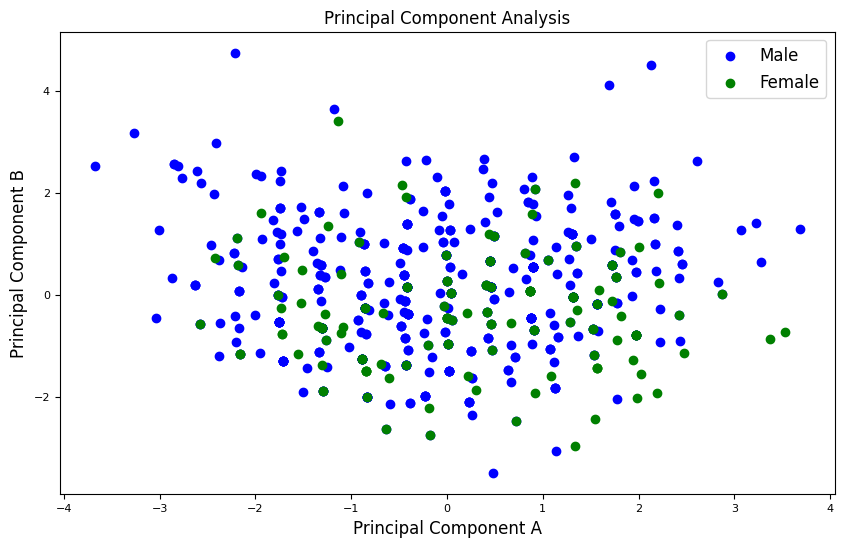
\includegraphics[width=0.5\linewidth]{images/PCA.png}
    \caption{Principal Component Analysis (PCA) where the coordinates of every point is dependent on the personality assessments of speakers based on two principal components (Principal Component A \& Principal Component B). The gender of each points corresponding to a speaker is indicated by colour.}
    \label{fig:ML_PCA}
\end{figure}

Principal Component Analysis was applied to project the five dimensions of the Big Five personality scores into a two dimensional plot where each point corresponds to an audio recording made up of the five scores. This was done to observe the impact of each one of the Big Five personality traits on the describe personality of a speaker. 
The plot, as illustrated in figure \ref{fig:ML_PCA}, includes two principal components which visualise approximately 66\% of the variance between the two genders while no significant separation between the gender groups is noticeable. 
The variance between the gender only increases to over 90\% when five components are used while it does not surpass 90\% when four components are calculated. Similarly, when assessing the impact of each personality trait on the principal components, it appears that to achieve higher representation of the variance, all Big Five traits are needed. This implies that indeed all five personality traits are necessary to provide a full picture of the described personality in the distinction between the genders. Following this reasoning, all personality traits scores are used as features to the adopted models which simultaneously reinforces the association of the Big Five personality traits and gender.

\subsection{Internal functionality of models}

This phase was implemented using Python's open-source Scikit-learn library which allows for the integration of machine learning models in code \citep{kramer2016scikit}. Five supervised learning classification algorithms were adopted for this purpose. The algorithms were used to assess the classification of personality scores assigned to an audio clip mapped to the respective gender of the speaker. The high level functionality of the algorithms involves the average personality perception scores for every audio clip across the 11 judges. These five scores per recording are the input features to the models as established in section \ref{sec:PCA} which are in turn classified into one of the binary gender classes.

In order to carry out the classification algorithms required to achieve bias detection in the dataset, a series of steps were followed.
Initially, in line with the structure of the dataset, the data was manipulated and adapted accordingly. This was accomplished through encoding the gender labels into binary digits. Label encoding is the process of relabelling each entry in the form of the binary numbers to be embedded into the algorithms.

In the procedure of training and testing a machine learning model, depending on the model adopted there are various hyperparameters which can be specified to optimise the model’s performance. To achieve such optimisation however, the process of hyperparameter tuning needs to be performed. Hyperparameter tuning is the method of tweaking the different parameters of an algorithm in order to maximise the algorithm performance for the project specific purpose using the relevant dataset. Preliminary testing of the models is used to evaluate the models under different hyperparameter combinations. As a result, through systematic assessment of the effectiveness of the models, the most favourable hyperparameters are determined. This is done on a model basis depending on the system’s purpose.

When dealing with machine learning models, cross-validation is a technique adopted to ensure reliability in the results while avoiding the occurrence of findings which do not represent the dataset and models as a whole.
Taking into consideration the shared speakers amongst the dataset’s recordings as well as the uneven representation of the two gender classes in the dataset, stratified group k-fold cross-validation is used. According to the process of k-fold cross validation, the training test is split into k subsets, known as folds, where in each of the k iterations all but one of the subsets are used to train the model while the remaining one is used to test it. By repeating this process, the whole dataset is tested while avoiding any overlap between train and test sets and simultaneously maintaining speaker separation.

In the context of the dataset, some of the featured audio recordings share a common speaker. To ensure that this does not negatively interfere with model performance and to avoid over-fitting while maintaining generalisable results, group splitting was used. This was incorporated to ensure a robust evaluation of the models since group splitting guarantees that any clips which include a shared speaker are maintained in same set split. As a result, the same speaker does not appear in both the training and testing sets leading to an honest output.
At the same time, stratified k fold takes into account the class imbalance in the data and applies the same proportional distribution of each class label in every one of the fold splits. This decision is endorsed by \citep{fontanari2022cross} who investigated the comparison of various cross-validation techniques and strategies and found that in the context of an imbalanced dataset, stratified cross-validation is most appropriate.

Returning to hyperparameter tuning, in this study, Grid Search Cross-validation was adopted. This method is used to automatically derive the optimal hyperparameters through exhausting all the possible hyperparameter combinations for a given model using a brute-force approach. Stratified group k-fold cross validation was specified as a parameter of the GridSearchCV function to be used during the hyperparameter tuning procedure. Accordingly, for every hyperparameter combination, the model was trained and tested k times while retrieving a performance metric for every fold and maintaining stratified group splits. The best hyperparameters for a model were thus defined by comparing the average performance metric over the various folds per hyperparameter set.
The performance metric adopted in this implementation was accuracy since the evaluation of the algorithm is performed using the Binomial test, discussed in section \ref{sec:Design_ML_eval}. 

The performance of the models was quantified both prior and post hyperparameter tuning. Considering the imbalance between classes present in the corpus the “class\_weight” hyperparameter was applied in both cases. The purpose of this parameter is to address the skew in class distribution by assigning different weights to the two binary classes. By giving more weight to the minority class during training, the algorithm can account for bias deriving from the imbalance. This setting is interpreted by the algorithm to assess the number of occurrences of each class in the set and adjust the weights according to the inverse proportion of their frequencies. This is attained by following the formula of:
\begin{equation}
\text{{class\*weight}} = \frac{n_{samples}}{{n_{classes}} \cdot {n_{class}}}
\end{equation}
where $n_{samples}$ is the number of samples in the input, $n_{classes}$ is the number of target labels, in this case 2 for the binary genders and $n_{class}$ is the frequency of each one of the two class labels.
While maintaining this hyperparameter fixed, various other hyperparameters were adjusted within the grid search process. Through the mandatory use of "class\_weight", assigning accuracy as the performance metric does not jeopardise the consideration of the class imbalance when adjusting the hyperparameters.

\subsection{The models \& their Hyperparameters}
The models adopted after hyperparameter tuning were implemented as follows where the mentioned hyperparameters are the ones differing from the defaults:
\begin{itemize}

\item The Logistic Regression algorithm models classification into a binary result and is executed through regression analysis. This process occurs using a logistic function which transforms the linear combination of the inputted features of the data and determines the probability score of which class the data belongs to based on the inputted features. Hence, it categorises the inputted instance based on the probability it belongs into one of the classes. Classification is achieved through a threshold which defines the probability at which classification is determined.

In terms of hyperparameters, the parameters specified for the Logistic Regression classifier in this implementation were "solver" and “class\_weight”. 
The hyperparameter "solver" signifies the algorithm defined in the optimisation. "liblinear" was the algorithm chosen for this project since it is well suited for binary classes and thus was deemed most effective during hyperparameter tuning. 

\item The K-Nearest Neighbours (KNN) classifier is an algorithm which operates by finding the k nearest instances derived from the dataset, on which the model is trained upon. These neighbours are compared to the input features for which a prediction is made. Depending on the distance between the neighbour values, the frequency of the class labels that belong to the k closest neighbours in the feature space is calculated. The class in which the majority of neighbours belong to defines the classification of the current input and finally a prediction is made. The KNN classifier does not consider the weight that the features have on the classification and thus behaves toward the values of all features in a similar way.

The number of the k nearest features which are considered in the algorithm is thus a determining factor of its performance. The number defined in this implementation as a hyperparameter is 7. It is deduced that considering 7 neighbours in order to make a classification, is optimal for this dataset. Another hyperparameter specified is “weights” which is set to follow the inverse of the distance between the weight points. This choice emphasises the neighbours which are closer while the ones further away have a smaller impact on the final classification.  


\item The Decision Tree classifier is constructed using tree structures which depending on the input features in the form of nodes lead to a classification outcomes in the form of leaves. This process is carried out by branches which act as rules that define the decision nodes and build a path towards the class labels, the leaves. The tree structures are formed by the training data being separated into subsets based on how the features define classification individually. At each node, a feature is chosen to determine the following node down the tree. This design allows for maximum benefit from each feature.
The hyperparameter “max\_depth” defined for the Decision Tree classifier is the maximum depth the tree nodes can reach. This parameter was set to 10 under hyperparameter tuning. According to “max\_depth”, the tree cannot grow to reach a depth of over 10 nodes from the root node in the case of the longest path to a leaf node. 

\item Random Forest Classifier is an algorithm which follows an interpretation that incorporates multiple Decision Tree classifiers to achieve an optimal prediction. The trees are defined using a set of different randomly selected subsets from the training data and the features on which they are trained on. Each one of the various trees define a unique method of classification corresponding to the selected features on which it was trained. Amongst the multiple classifications of the input features, the most commonly inferred label is returned.

As discussed previously, in this implementation, the parameter “class\_weights” is set to “balanced” to account for the dataset’s imbalance. Another hyperparameter is the number of estimators is adjusted which is a hyperparameter determining how many decision trees are trained individually and are included in the decision of the classifier. The higher the number of the estimators, the more robust the model is expected to be. For this project, this hyperparameter is set to 200 as it seemed most effective in terms of performance. Lastly, similarly to the Decision Tree classifier, the “max\_depth” parameter was specified but in this case it was set to 10.

\item The Support Vector Machine (SVM) algorithm, often used for classification, relies on the construction of a hyperplane in a multidimensional space which acts as a separator between the different classes. The hyperplane defines a separation between the two labels and is designed with goal to increase the distance at which the class separation takes place as much as possible. The greater the separation between the closest data points from each class, the more robust the algorithm is in classifying. Each prediction is made by detecting the side of the plane in which the instance falls into.

A key hyperparameter in this algorithm is the regularisation parameter, "C". This parameter regulates the relation between the margin which determines the hyperplane and the potential for misclassification.
Another hyperparameter is the kernel type. This is the type of boundary used in the classification of features and determines how similar different entries are in the feature space. In this project, "C" is set to 5 and the polynomial kernel is adopted. When specifying a polynomial kernel, the degree of the polynomial kernel function can be applied which controls how complex the decision boundary is which was specified as 5. The polynomial kernel function is defined as:
\begin{equation}
K(a, b) = (a \cdot b + c)^d
\end{equation}
where $a$ and $b$ are the input vector, $d$ is the degree of the polynomial kernel and $c$ is a constant.
\end{itemize}

Having established the ideal hyperparameters for each one of the models, the models along with their optimal hyperparameters were trained and tested once more using stratified group k fold cross validation.

\subsection{Evaluation}\label{sec:Design_ML_eval}

The models’ performance was output in the form of a confusion matrix as well as the respective $F_1$, precision, recall and accuracy scores as these are metrics most appropriate when dealing with uneven class distribution. Their formulas for precision and recall are as follows:
\begin{equation}
\text{Precision} = \frac{\text{True Positives}}{\text{True Positives} + \text{False Positives}}
\end{equation}
\begin{equation}
\text{Recall} = \frac{\text{True Positives}}{\text{True Positives} + \text{False Negatives}}
\end{equation}
where $\text{Precision}$ is the ratio of the true positive results of the model to the total predicted positives and $\text{Recall}$ is the ratio of true positive outcomes to the total real positive labels. 
The $F_1$ score is a metric associated to the confusion matrix, which is a combination of the recall and precision scores with the following formula:
\begin{equation}
\text{$F_1$}= 2 \times \frac{\text{Precision} \times \text{Recall}}{\text{Precision} + \text{Recall}}
\end{equation}

The performance of a model is optimal if the $F_1$ score is 1. The $F_1$ score was chosen as a metric to be considered in this case due to its versatility when dealing with imbalanced datasets \citep{kong2019hyperparameter}.
The accuracy is calculated based on the number of correctly classified entries in comparison to the total number of predictions made:
\begin{equation}
    \text{Accuracy} = \frac{\text{True Positives + True Negatives}}{\text{Total predictions}}
\end{equation}


To establish  the credibility of the algorithms’ outcomes, the Binomial test was adopted. The Binomial test is used for the comparison of the observed counts of the inputted binary categories against the hypothesised counts. In this case, Binomial tests were executed for every one of the modelled algorithms. This was done to examine the models' predicted classifications against and the likelihood of obtaining the same performance in values by chance. The tests then examine whether the observed outcomes of the models differ to a significant extent from the hypothesis.
This was done by inputting the number of correctly predicted labels against the probability of making these predictions by chance according to the structure of the dataset. In this case, the prior probability was calculated using the sum of squares of the the male and female probabilities. The robustness of the models' results is reflected on the p-value output of the Binomial tests where statistical significance signifies the trustworthiness of the predicted model classifications.
The Binomial test formula adapted is:
    \begin{equation}
    p= \sum_{i=0}^{k} \binom{n}{i} p^i (1-p)^{n-i}
    \end{equation}
where $k$ is the number of correctly predicted classifications, $n$ is the number of total predictions and $p$ is the probability of success as a result of a single classification.

Additionally, the models' performance for the accuracy metric was compared using a Student's t test with the prior probability of 66\% used for the Binomial test as well. T test were also computed for the metrics of F1, precision and recall scores but instead compared the with probability of the positive class. The probability of the positive class was chosen based on the nature of precision and recall and thus F1 score as well which takes into account the class imbalance.
These t-test were used by considering the scores of the metric for every fold against the positive class probability. The use of this tests allowed for the inclusion of the performance metrics other than accuracy and the use of the scores from the different folds which represents the standard deviation between these scores. Bonferroni correction was also used for every performance metric giving an alpha of 0.01 as there are five models.

\section{Audio Processing  \& Within Gender Assessment}

In accordance to chapter \ref{chap:Analysis}, in order to investigate the impact of gender stereotypes on within gender judgement in this corpus, based on a measure which often relates to femininity,  fundamental frequency $f_0$ is used.

For this to be achieved, the fundamental frequency is extracted from each of the audio files.

\subsection{Feature Extraction}

The first step required in this stage was the extraction of the vocal features from each one of the audio clips. For this purpose, the openSMILE tool was employed \citep{Eyben2010}. OpenSMILE is an open-source toolkit which has the functionality of extracting audio features from speech and is adopted in the context of automatic emotion recognition. Acknowledging the use of fundamental frequency and its relation with this project discussed in previous sections, openSMILE was chosen to extract the fundamental frequency from the recordings in the corpus.
In order to use openSMILE to perform the feature extraction, a configuration file was applied. OpenSMILE requires configuration files to specify necessary information to perform the extraction such as the input and output files as well as feature sets and parameters. The configuration file used in this case follows the feature set defined in The Interspeech 2009 Emotion Challenge \citep{schuller2009interspeech} which was dedicated on human emotion recognition derived from speech.

The vector of fundamental frequency values extracted from the recordings is representative of the algorithm and the sampling rate of the audio recording in terms of the time frames. According to the used configuration file, frame segmentation of the audio signal results into overlapping frames of 25ms each where a new frame starts after 10ms leading to the overlapping windows used to process the audio clips.
Consequently, the number of fundamental frequency values corresponds to the number of time frames. Under this project, each recording has approximately 1000 values, where a substantial part displays instances of zero values which are attributed to breaks in speech.
Having gathered the fundamental frequency vectors of every audio clip, the average fundamental frequency of every one of the recordings was calculated in order to allow for comparison and representation of the clips. The zero values were omitted from this calculation to produce representative metrics as they represent silence in the breaks between speech.

\subsection{Within gender inter-rater agreement}
In accordance to the inter-rater agreement computed in section \ref{sec:design_agreement}, the process is replicated under the condition of using only speakers of one gender. The inter-rater agreement is used to find the reliability in the dataset specifically when addressing within gender comparisons.

\subsection{Within gender comparison}

Consistent section \ref{sec:Within_gender}, within gender assessment hypotheses incorporate the influences of gender stereotypes manifested beyond gender distinction. Their relationship with gender bias entails that fundamental frequency in association with gender should indicate an effect on personality assessments even within gender. 

As a result, the comparisons made to assess this involved the average fundamental frequency against the personality score per recording for every personality trait individually. Spearman’s rank correlation coefficient and the corresponding p-value are derived for every trait separately to examine this effect. Through this process, the correlation between the fundamental frequency of the speaker’s voice and the average score among the judges for that audio clip is calculated.
Therefore, the response to gender stereotypes and the significance of the findings can be evaluated.
The formula for Spearman’s rank is as follows:

\begin{equation}
\rho = 1 - \frac{6\sum d_i^2}{n(n^2 - 1)}
\end{equation}

where $\rho$ denotes the Spearman’s rank correlation coefficient, $d_i$ is the difference between the ranks of the pairs of values of every correlation and n is the number of observations which are included in the calculation. The output for every personality trait comparison was the correlation coefficient, $\rho$, and the p-value. The correlation coefficient is a value between -1 and 1 where 1 suggests a perfect positive monotonic relationship while -1 indicates a perfect negative monotonic relationship. A $\rho$ value of 0 represents no monotonic correlation at all amongst the two variables. In this test, an association between the fundamental frequency and personality scores following the hypothesis would imply a positive monotonic relationship between the variables. The metric of Spearman's rank was specifically chosen to assess this data as it is not sensitive to outliers in the case of potential audio distortion or expressive emotion in the speaker's voice.

In a similar manner to section \ref{sec:Implementation_stat}, Bonferroni correction was likewise exercised to account for the multiple comparisons due to the different personality scores. This resulted to an alpha value of 0.01.

\section{Summary}
This chapter examined both the design of the project in terms of the procedures it follows at a high level but also elaborated upon the implementation of the various stages including the technical tools used and the specific implementation choices made. The statistical decisions utilised throughout the project were defined along with how they fit into the nature of the dataset. Moreover, to illustrate the detection of bias through machine learning, a list the classification models chosen is provided and their relationship with the data points from the corpus. The implementation specific machine learning choices like hyperparameter tuning decisions were outlined. Additionally, a method of audio extraction and manipulation is discussed which is attempted to explore the concept within gender inferences. Finally, for every section of the project, the processes employed to assess the outcomes and reliability of the experiments were presented.
%==================================================================================================================================
\chapter{Results}\label{chap:Results}
This chapter is dedicated to the project's findings at every phase described in chapter \ref{chap:Design_Implementation}.

\section{Statistical Analysis}

\subsection{Inter-rater agreement}\label{sec:Results_agreement}

\begin{table}[b]
%\tt 
\centering
\rowcolors{2}{}{gray!3}
\begin{tabular}{llll}
%\toprule 
\small{\textbf{Big Five Traits}} & \small{\textbf{Reliability Coeff.}} & \small{\textbf{Female Reliability Coeff.}}  & \small{\textbf{Male Reliability Coeff.}}\\ \hline%\midrule
Extraversion        & 0.804054    & 0.814321    & 0.803662                     \\
Agreeableness       & 0.595927    & 0.544303    & 0.597404                     \\
Conscientiousness   & 0.567465    & 0.517704    & 0.553239                     \\
Neuroticism         & 0.604638    & 0.516347    & 0.616003                     \\
Openness            & 0.103023    & 0.255115    & 0.052161   
\end{tabular}
\vspace{10pt}
\caption{Inter-rater agreement Reliability coefficients: Spearman-Brown Reliability Coefficients for the Big Five personality traits for each group of all speakers, female speakers and male speakers calculated using the average Spearman's rank rho including the personality judgements between 11 judges.}
\label{table:StatAnalysis_brown}
\end{table}

The inter-rater agreement according to the Spearman-Brown reliability coefficient presents the agreement between judges and thus the reliability in the data. As a result, an evaluation of reliability within the corpus is performed.
Through execution of the Spearman-Brown formula, the greatest reliability in judgements was signified for the traits of perceived Extraversion ($\rho$ = 0.80), followed by Neuroticism ($\rho$ = 0.60) as displayed in table \ref{table:StatAnalysis_brown}.
According to \citet{fleiss1981measurement}, it was reported that inter-rater agreement within the range 0.75-1 is excellent, agreement within the range 0.40-0.75 is fair to good and poor agreement is found under 0.40. 
Similar reliability was found between Extraversion and the traits of Agreeableness ($\rho$ = 0.60) and Conscientiousness ($\rho$ = 0.57) which suggests a fair to good result.
The only trait that revealed very poor reliability was Openness which was substantially lower than all traits ($\rho$=0.10).

In terms of the reliability when considering speakers of a single gender, within gender inter-rater agreement is displayed in table \ref{table:StatAnalysis_brown}. 
Inter-rater agreement when assessing female speakers was highest for Extraversion ($\rho$ = 0.81) and was second highest for Agreeableness ($\rho$ = 0.54) while agreement was lowest for Openness ($\rho$ = 0.26). The rest of the traits employed a similar agreement around $\rho$ = 0.52.
As it concerns male speakers, the agreement for Agreeableness ($\rho$ = 0.60), Conscientiousness ($\rho$ = 0.55) and Neuroticism ($\rho$ = 0.62) were slightly higher. However, Openness had very low reliability at $\rho$ = 0.05.
Similarities are prominent between the within gender reliability and the collective reliability for most traits.
For both genders, the agreement in Extraversion was evaluated to be very close to the agreement when considering all audio clips. For the traits of Agreeableness, Neuroticism and Conscientiousness, slightly higher agreement was found when comparing scores assigned to male speakers in comparison to female speakers. The opposite effect, but to a greater extent, is observed for Openness where agreement for female speakers reliability is $\rho$ = 0.26 while for male speakers it is $\rho$ = 0.05. 


\begin{figure}[h]
        \centering
        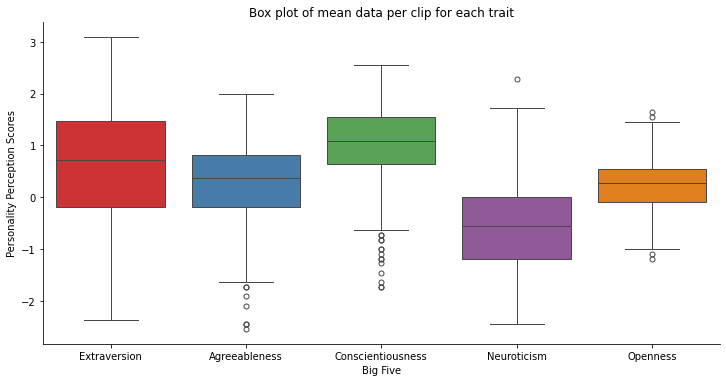
\includegraphics[width=0.90\linewidth]{images/distribution_traits.png}
        \caption{A series of Box plots illustrating the average personality assessment scores given to audio recordings by the judges.}
        \label{fig:distribution_traits}
    \end{figure}
    
\begin{table}[h]
    \centering
    %\tt 
    \rowcolors{2}{}{gray!3}
    \begin{tabular}{lllll}
        %\toprule 
        \textbf{Big Five Traits} & \textbf{Minimum}           & \textbf{Median}            & \textbf{Maximum}          & \textbf{Standard Deviation} \\ \hline
        Extraversion             & -3                         & 1                          & 4                         & 1.325566                    \\
        Agreeableness            & -3                         & 0                          & 2                         & 0.914476                    \\
        Conscientiousness        & -2                         & 1                          & 3                         & 0.889433                    \\
        Neuroticism              & -3                         & -1                         & 3                          & 1.097422                    \\
        Openness                 & -2                         & 0                          & 2                         & 0.533917                    \\
    \end{tabular}
    \vspace{10pt}
    \caption{Summary Statistics of all scores per personality trait: Median, Minimum, Maximum, and Standard Deviation ($\sigma$).}
    \label{table:Pitch_Gender_values}
\end{table}

\subsection{Gender differences}\label{sec:Results_gender_differences}

\begin{table}[h]
\centering
%\tt 
\rowcolors{2}{}{gray!3}
\begin{tabular}{lll}
%\toprule 
\textbf{Big Five Traits} & \textbf{T statistic} & \textbf{p-value} \\ \hline%\midrule
Extraversion             & 0.841339             & 4.004731e-01     \\
Agreeableness            & 5.385740             & 1.015605e-07     \\
Conscientiousness        & 6.072088             & 2.168292e-09     \\
Neuroticism              & 3.219771             & 1.348044e-03     \\
Openness                 & 4.129047             & 4.127029e-05     \\ 
\end{tabular}
\vspace{10pt}
\caption{Student's t-test results for the comparison of the female against male average personality scores per audio recording per Big Five trait.}
\label{table:StatAnalysis_ttest}
\end{table}

\begin{figure}
    \centering
    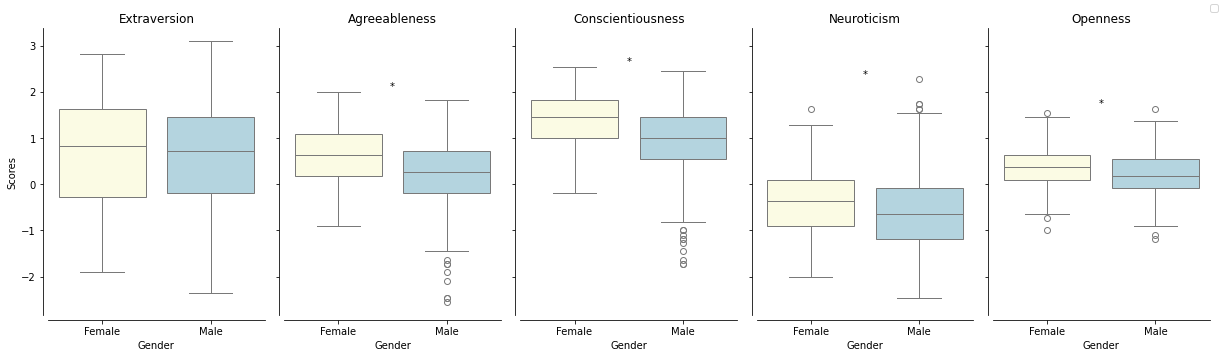
\includegraphics[width=0.99\linewidth]{images/genderSplit_boxplot.png}
    \caption{A series of Box plots illustrating the average personality assessment scores given to audio recordings by the judges. Each plot represents a Big Five personality trait under which the scores were assigned which are separated into the two boxes dedicated to the binary genders. "*" indicators suggest statistical significance according to the t-test results between the genders per trait.}   
    \label{fig:StatAnalysis_boxplot}
\end{figure}

To statistically analyse the relationship between the personality scores corresponding to the two genders, two-sample student’s t-tests were employed to compose a comparison between the average personality assessment scores between the female and male speaker groups. These tests yielded the t-statistic between the two genders as well as the p-value, one for every personality trait. As illustrated in table \ref{table:StatAnalysis_ttest}, there is a positive t-statistic for all personality traits which indicates a difference between the two groups. With regard to the statistical significance of the outcomes, it was deduced that for the attribute of Extraversion the result was not significant (t = 0.84 ,p > 0.01). This is evident as the p-value is greater than the threshold of 0.01 which was the computed alpha value as a result of the Bonferroni correction.
The remaining four traits were all found to be statistically significant and the greatest gender variation being attributed to the trait of Conscientiousness (t = 6.07 , p < 0.01) followed by Agreeableness (t = 5.39 , p < 0.01), Openness (t = 4.13 , p < 0.01) and finally Neuroticism (t = 3.22 , p < 0.01).


\section{Machine Learning}\label{sec:Results_ML}

\begin{table}[h]
\centering
%\tt 
\rowcolors{2}{}{gray!3}
\resizebox{\textwidth}{!}{
\begin{tabular}{lll}
\textbf{Models}           & \textbf{Binomial test p-value - before} & \textbf{Binomial test p-value - after}  \\ \hline
Logistic Regression      & 1.807214e-01              & 1.807214e-01                   \\
Random forest classifier & 4.029465e-01              & 7.697149e-01                   \\
Decision tree classified & 1.432261e-01              & 1.549483e-01                   \\
SVM                      & 2.952793e-02              & 2.306020e-08                   \\
K-nearest neighbours     & 6.192301e-14              & 1.195554e-13                   \\ 
\end{tabular}
}
\vspace{10pt}
\caption{Binomial Test p-value for the five classification models before and after hyperparameter tuning.}
\label{table:Binomial_Test_before_after}
\end{table}

\begin{table}[h]
  \centering
  \caption*{Confusion Matrices post Hyperparameter tuning}
  %\tt
    \renewcommand{\arraystretch}{1.5} % Adjust the value for increased row spacing
    \begin{tabular}{
    >{\columncolor[HTML]{FFFFFF}}l 
    >{\columncolor[HTML]{EFEFEF}}l |
    >{\columncolor[HTML]{FFFFFF}}l 
    >{\columncolor[HTML]{FFFFFF}}l }
                                                                                                                                       & \cellcolor[HTML]{FFFFFF}                    & \multicolumn{2}{l}{\cellcolor[HTML]{FFFFFF}\textbf{Predicted Class}}         \\
    \multicolumn{1}{l|}{\cellcolor[HTML]{FFFFFF}\textbf{Model}}                                                                        & \cellcolor[HTML]{FFFFFF}\textbf{True Class} & \multicolumn{1}{l|}{\cellcolor[HTML]{FFFFFF}\textbf{Male}} & \textbf{Female} \\ \hline
    \multicolumn{1}{l|}{\cellcolor[HTML]{FFFFFF}}                                                                                      & Male                                        & \multicolumn{1}{l|}{\cellcolor[HTML]{FFFFFF}348}           & 155             \\
    \multicolumn{1}{l|}{\multirow{-2}{*}{\cellcolor[HTML]{FFFFFF}Logistic Regression}}                                                 & Female                                      & \multicolumn{1}{l|}{\cellcolor[HTML]{FFFFFF}43}            & 94              \\ \hline
    \multicolumn{1}{l|}{\cellcolor[HTML]{FFFFFF}}                                                                                      & Male                                        & \multicolumn{1}{l|}{\cellcolor[HTML]{FFFFFF}356}           & 147             \\
    \multicolumn{1}{l|}{\multirow{-2}{*}{\cellcolor[HTML]{FFFFFF}Random Forest Classifier}}                                            & Female                                      & \multicolumn{1}{l|}{\cellcolor[HTML]{FFFFFF}72}            & 65              \\ \hline
    \multicolumn{1}{l|}{\cellcolor[HTML]{FFFFFF}}                                                                                      & Male                                        & \multicolumn{1}{l|}{\cellcolor[HTML]{FFFFFF}391}           & 112             \\
    \multicolumn{1}{l|}{\multirow{-2}{*}{\cellcolor[HTML]{FFFFFF}\begin{tabular}[c]{@{}l@{}}Decision Tree \\ Classifier\end{tabular}}} & Female                                      & \multicolumn{1}{l|}{\cellcolor[HTML]{FFFFFF}85}            & 52              \\ \hline
    \multicolumn{1}{l|}{\cellcolor[HTML]{FFFFFF}}                                                                                      & Male                                        & \multicolumn{1}{l|}{\cellcolor[HTML]{FFFFFF}443}           & 60              \\
    \multicolumn{1}{l|}{\multirow{-2}{*}{\cellcolor[HTML]{FFFFFF}Support Vector Machine}}                                              & Female                                      & \multicolumn{1}{l|}{\cellcolor[HTML]{FFFFFF}90}            & 47              \\ \hline
    \multicolumn{1}{l|}{\cellcolor[HTML]{FFFFFF}}                                                                                      & Male                                        & \multicolumn{1}{l|}{\cellcolor[HTML]{FFFFFF}476}           & 27              \\
    \multicolumn{1}{l|}{\multirow{-2}{*}{\cellcolor[HTML]{FFFFFF}K-nearest neighbours}}                                                & Female                                      & \multicolumn{1}{l|}{\cellcolor[HTML]{FFFFFF}105}           & 32              \\ 
    \end{tabular}
    \vspace{10px}
  \caption{Confusion Matrices for the five algorithms after hyperparameter tuning. The rows represent the true class labels of the samples and the columns represent the predicted class labels as male and female.}
  \label{table:confusion_matrices}
\end{table}

\begin{figure}
    \centering
    \caption*{Bar Charts for model performance scores post Hyperparameter tuning}
    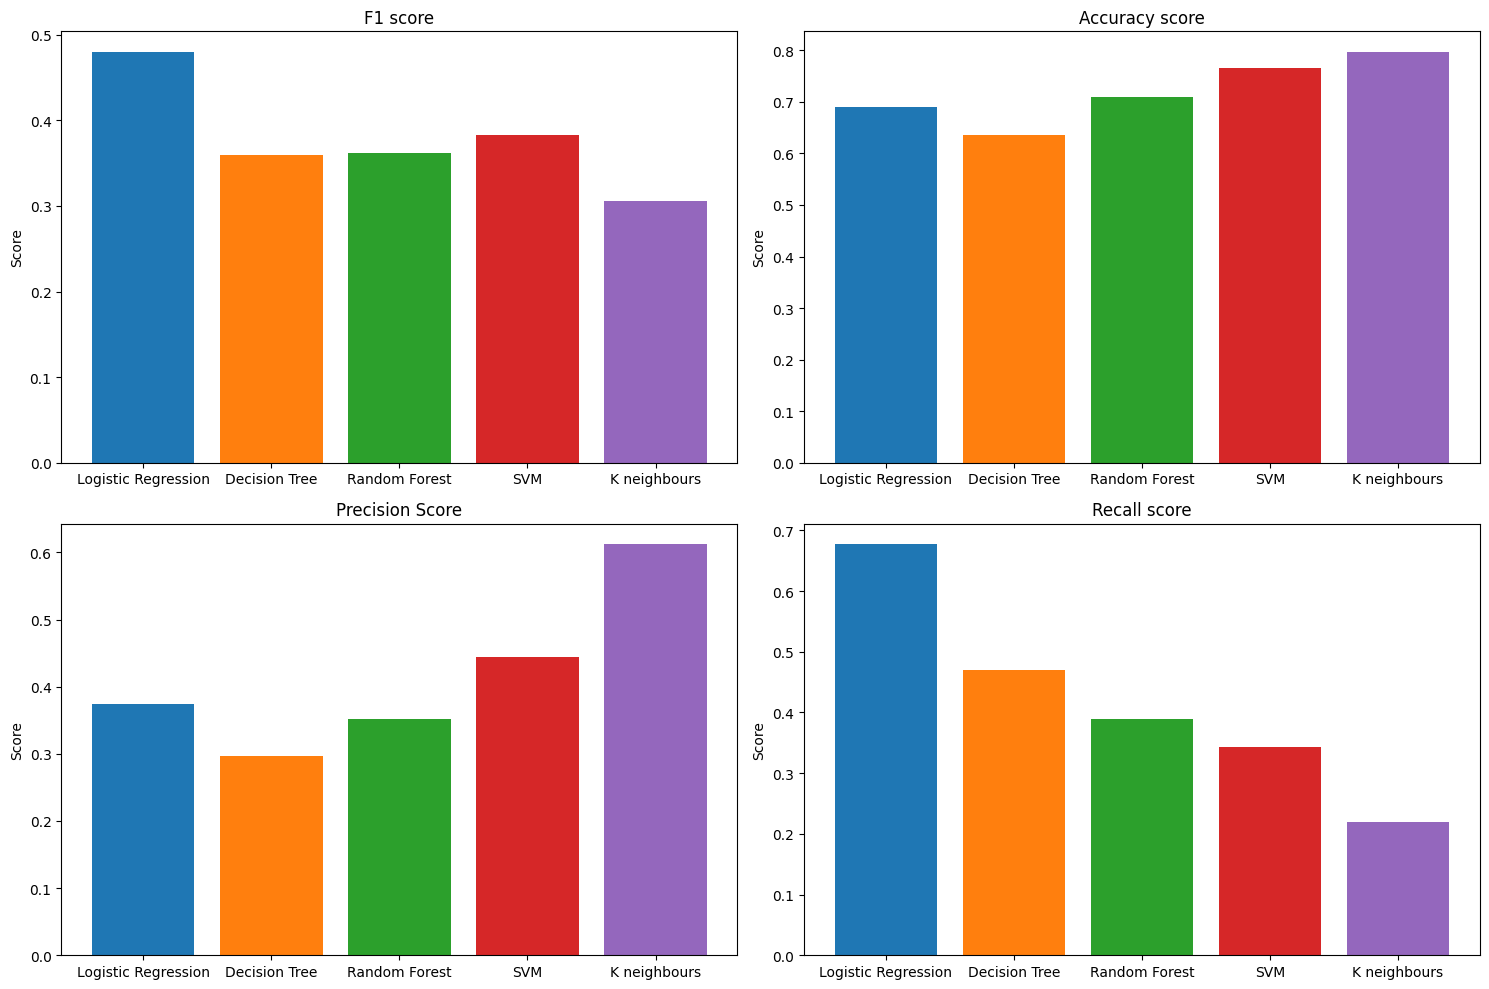
\includegraphics[width=1\linewidth]{images/models_barcharts_performancemetrics.png}
    \caption{Bar charts for every performance metric for each classification algorithm's performance post hyperparameter tuning. The "*" indicators suggest statistical significance as a result of Student's t tests between the metric over the k-folds and the prior probability of 66\% for accuracy and the probability of the positive class for the rest.}
    \label{fig:model_barcharts_performancemetrics}
\end{figure}

In the Machine Learning phase, the five models described in section \ref{sec:Implementation_ML} were trained and tested using the corpus and optimised using hyperparameter tuning. The models were evaluated through their performance based on their corresponding confusion matrices, illustrated in table \ref{table:confusion_matrices}, as well as the calculated $F_1$, accuracy, precision and recall scores. To establish the reliability of the models' outcomes the confusion matrices were implemented into Binomial tests to determine the model performance in comparison to what the performance would have been by chance. The Binomial test p-values are presented in table \ref{table:Binomial_Test_before_after} both before and after hyperparameter tuning. The only algorithms which were found to be statistically significant are the Support Vector Machine (accuracy = 0.77, $F_1$ = 0.38, precision = 0.44, recall = 0.34, p < 0.01) and K-nearest neighbours (accuracy = 0.80, $F_1$ = 0.31, precision = 0.61, recall = 0.22, p < 0.01). 
Despite the rest of the algorithms not being statistically significant, greater classification performance under the $F_1$ score was computed for the Logistic Regression model (accuracy = 0.69, $F_1$ = 0.48, precision = 0.37, recall = 0.69, p > 0.01). In comparison to the models prior to hyperparameter tuning, the optimisation using hyperparameter tuning appears to have improved the results since the Support Vector Machine gained statistical significance through the new hyperparameters.
The performance metrics post hyperaperameter optimisation are illustrated in \ref{fig:model_barcharts_performancemetrics}. The figure presents the performance of all models along with an indicator for statistical significance under Student's t-tests for each metric over the k folds in comparison to the prior probability of 66\% for accuracy and the probability of the positive class for the rest of the metrics. No significant difference was found between the performance of any model and the respective prior probability.

\section{Audio Processing  \& Within Gender Assessment}
In the investigation of within gender impacts of gender stereotypes, the correlations between fundamental frequency $f_0$ and personality perception were assessed. 

Audio feature extraction as well as student’s t-test were applied to assess the the effect of gender stereotypes on within gender inferences of personality perception. 
In consequence, the average extracted fundamental frequency $f_0$ was extracted per audio recording.
Initially, to compare the two genders, summary statistics of the fundamental frequency per gender were used which are displayed in table \ref{table:Pitch_Gender_values}. The results present higher overall scores in the case of female speakers (min = 117.66 Hz, mean = 173.45 Hz, max = 284.00 Hz, $\sigma$ = 28.44) whereas male speakers were assigned lower scores with the exception of maximum $f_0$ (min =  77.29 Hz, mean = 146.47 Hz, max = 367.32 Hz, $\sigma$ = 41.90). Recordings of male speakers also displayed higher average standard deviation of fundamental frequency $f_0$ in comparison to female speakers. 

Regarding the comparison between the two genders employed through the t-test (t = 7.10, p =  3.53e-12), the results indicate a statistically significant variation between the fundamental frequency of male and female speakers.

\subsection{Within Gender Assessment}


\begin{table}[h]
\centering
%\tt 
\rowcolors{2}{}{gray!3}
\begin{tabular}{lllll}
%\toprule 
\textbf{Gender} & \textbf{Mean $f_0$} & \textbf{Minimum $f_0$} & \textbf{Maximum $f_0$} & \textbf{Standard Deviation}\\ \hline
Female          & 173.450310         & 117.656982            & 283.996488            & 28.437971                   \\
Male            & 146.466992         & 77.286834             & 367.320230            & 41.903651                   \\ 

\end{tabular}
\vspace{10pt}
\caption{Summary Statistics of Fundamental Frequency $f_0$ values: Mean, Minimum, Maximum, and Standard Deviation (Hz).}
\label{table:Pitch_Gender_values}
\end{table}


\begin{figure}[h]
    \centering
    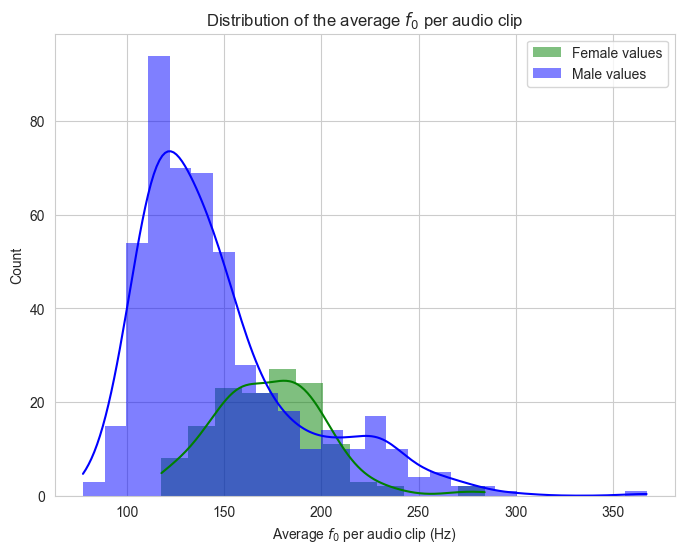
\includegraphics[width=0.5\linewidth]{images/distribution_genders_pitch.png}
    \caption{Distribution of average fundamental frequency $f_0$ values per audio recording for the two gender groups.}
    \label{fig:distribution_f0}
\end{figure}

\begin{figure}[h]
    \centering
    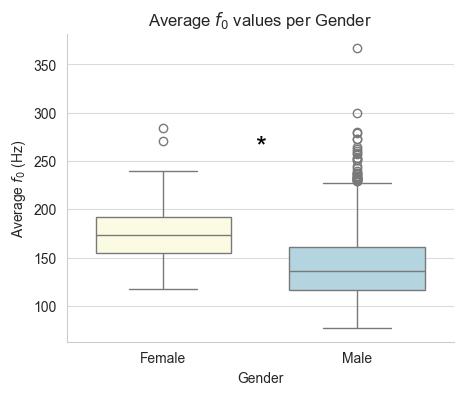
\includegraphics[width=0.6\linewidth]{images/boxplot_genders_f0.png}
    \caption{Box plot illustrating the average $f_0$ values per gender with significant difference according to a t test indicated by '*'.}
    \label{fig:f0_perGender_boxplot}
\end{figure}

\begin{figure}[h]
    \centering
    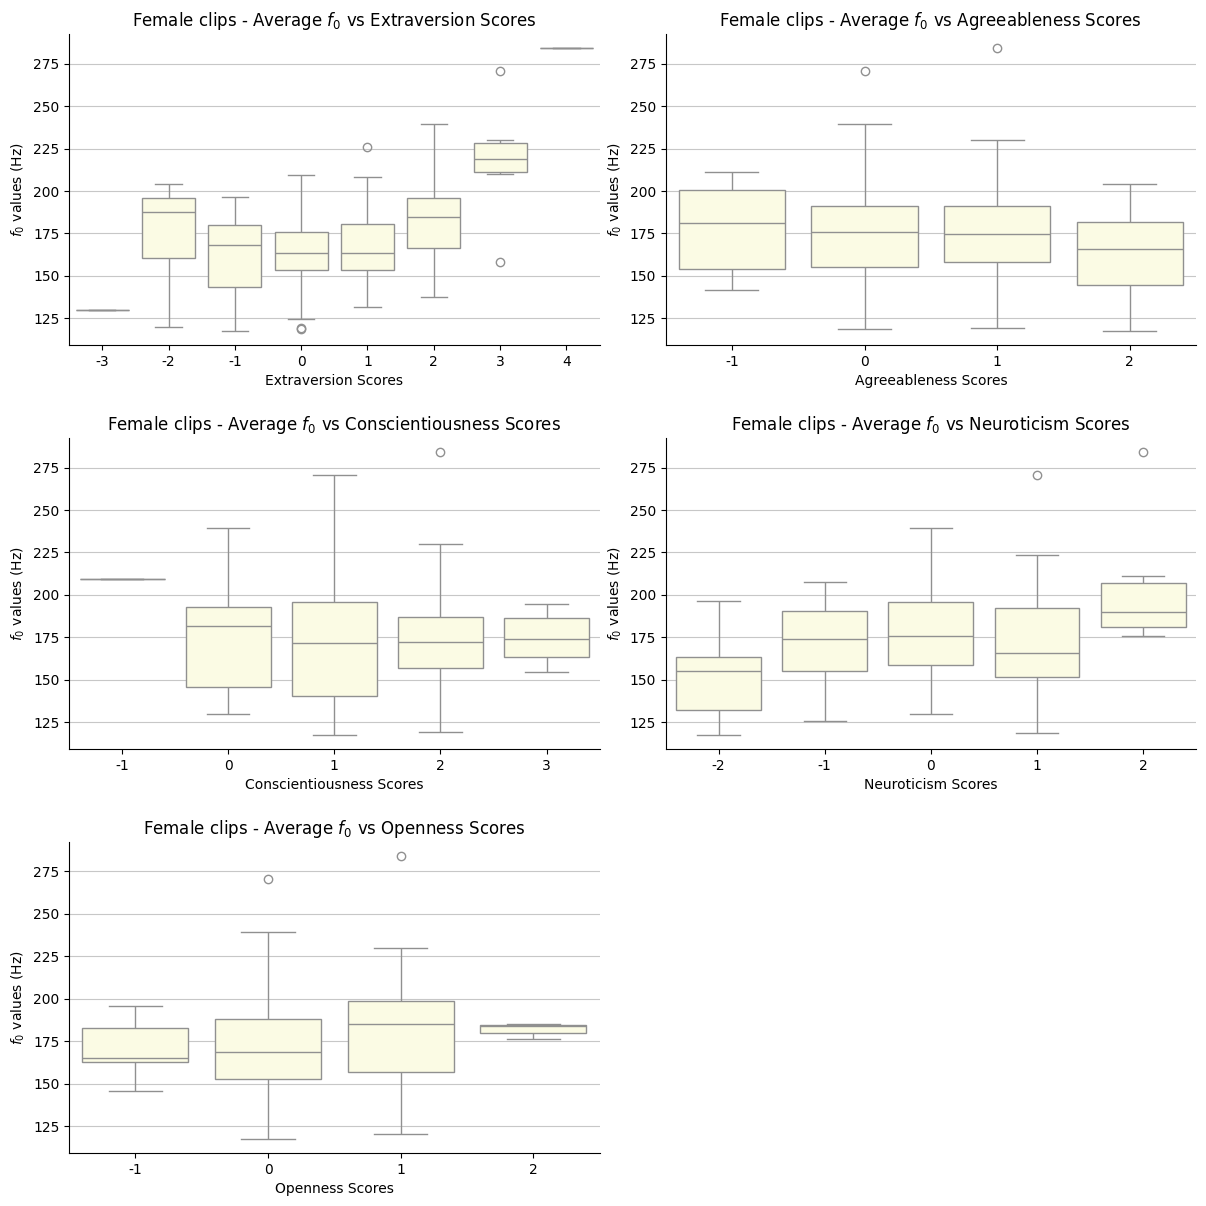
\includegraphics[width=0.99\linewidth]{images/female_audio_boxplot.png}
    \caption{A series of Box plots illustrating the range of average $f_0$ values corresponding to each personality perception score for a specific trait assigned to female speakers.}
    \label{fig:female_audio_boxplot}
\end{figure}

\begin{figure}[h]
    \centering
    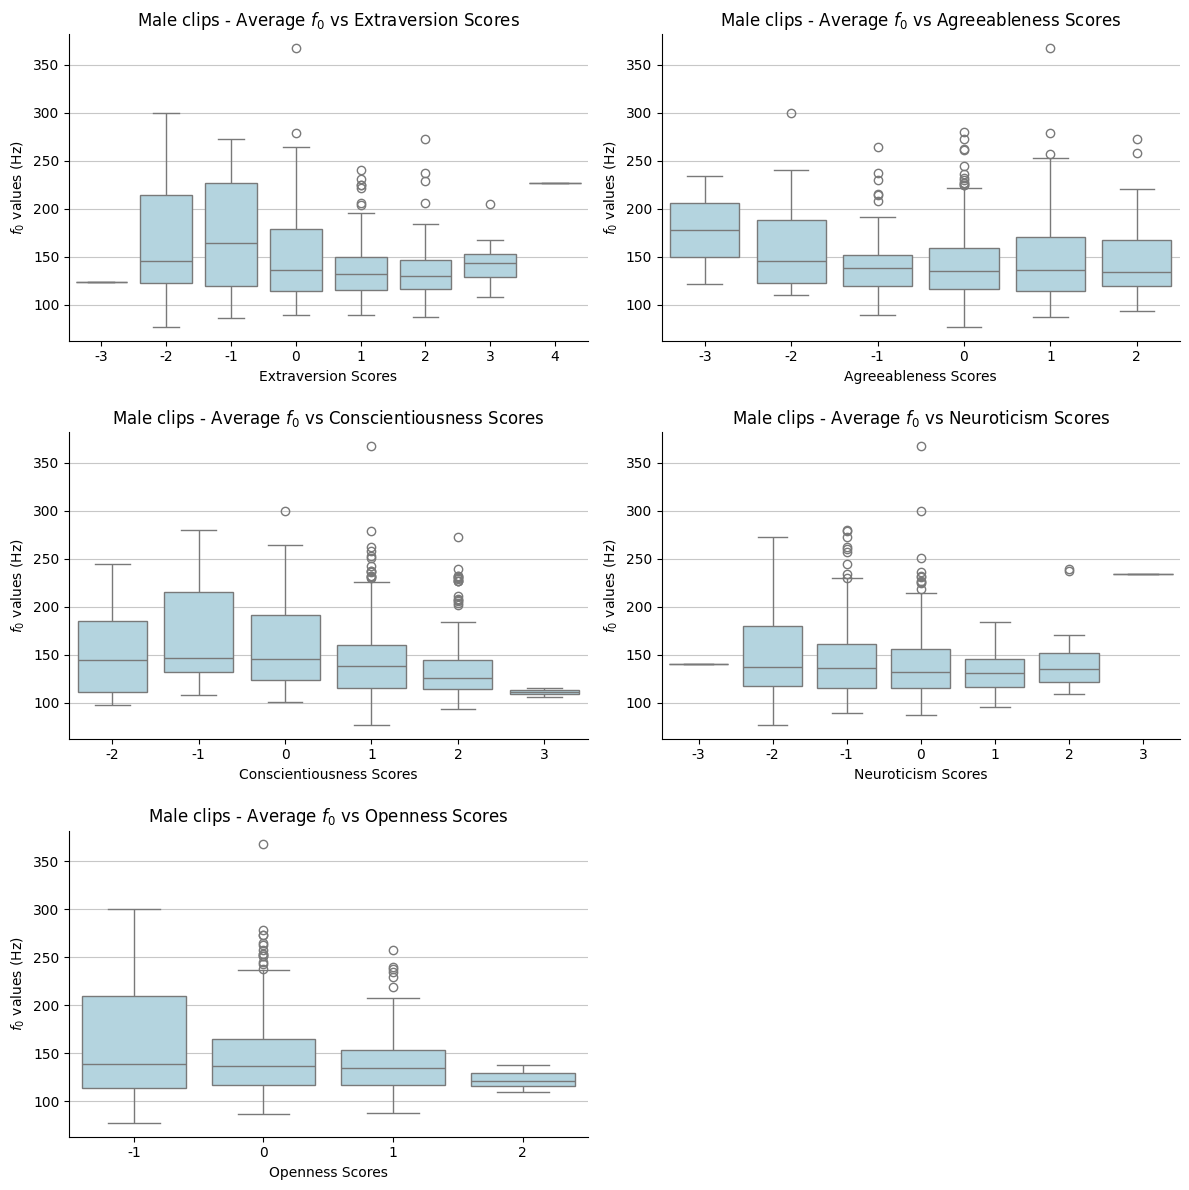
\includegraphics[width=1\linewidth]{images/male_audio_boxplot.png}
    \caption{A series of Box plots illustrating the range of average $f_0$ values corresponding to each personality perception score for a specific trait assigned to male speakers.}
    \label{fig:male_audio_boxplot}
\end{figure}

\begin{table}[h]
\centering
\caption*{Female speakers $f_0$ vs trait score correlation}
%\tt 
\rowcolors{2}{}{gray!3}
\begin{tabular}{lll}
%\toprule 
\textbf{Big Five traits} & \textbf{Spearman's rank $\rho$} & \textbf{p-value} \\ \hline%\midrule
Extraversion             & 0.299961                     & 0.000369         \\
Agreeableness            & -0.108466                    & 0.207071         \\
Conscientiousness        & -0.008762                    & 0.919055         \\
Neuroticism              & 0.270054                     & 0.001416         \\
Openness                 & 0.159689                     & 0.062327         \\ 
\end{tabular}
\vspace{10px}
\caption{Spearman's Rank Coefficients comparing the fundamental frequency $f_0$ against the average personality perception score assigned to an audio clips of female speakers for every recording per Big Five trait.}
\label{table:Audio_spearman_female}
\end{table}

\begin{table}[h]
\centering
\caption*{Male speakers $f_0$ vs trait score correlation}
%\tt 
\rowcolors{2}{}{gray!3}
\begin{tabular}{lll}
%\toprule 
\textbf{Big Five traits} & \textbf{Spearman's rank $\rho$} & \textbf{p-value} \\ \hline%\midrule
Extraversion             & -0.166116                     & 0.000188         \\
Agreeableness            & -0.00446                    & 0.920685         \\
Conscientiousness        & -0.217335                    & 0.000001         \\
Neuroticism              & -0.071829                     & 0.108316         \\
Openness                 & -0.040626                     & 0.364172         \\ 
\end{tabular}
\vspace{10px}
\caption{Spearman's Rank Coefficients comparing the fundamental frequency $f_0$ against the average personality perception score assigned to an audio clips of male speakers for every recording per Big Five trait.}
\label{table:Audio_spearman_male}
\end{table}

Spearman’s rank was the metric used to determine the within gender relation of fundamental frequency and personality perception scores per personality trait. Spearman’s rank correlation coefficients were calculated for every one of the Big Five traits within one gender group at a time. The coefficients of these calculations represent the relationships between the average fundamental frequency and personality perception score assigned to speakers for all audio clips. The results are presented in tables \ref{table:Audio_spearman_female} and \ref{table:Audio_spearman_male} where for female speakers the traits of Extraversion ($\rho$ = 0.30, p < 0.01) and Neuroticism ($\rho$ = 0.27, p <0.01) employ statistically significant results along with a positively correlated relationship between the the trait scores and $f_0$. Meanwhile, the traits of Agreeableness ($\rho$ = -0.11, p > 0.01) and Conscientiousness ($\rho$ = -0.01 , p > 0.01) have insignificant and negatively correlated outputs while the correlation for Openness is insignificant ($\rho$ = 0.16 , p > 0.01) but positively correlated. For male speakers, the results are substantially different as all correlations are negative. The traits of Extraversion ($\rho$ = -0.17, p < 0.01) and Conscientiousness ($\rho$ = -0.21, p < 0.01) are the only traits under which the correlation yielded statistical significance.

These results are accompanied by the figures \ref{fig:female_audio_boxplot} and \ref{fig:male_audio_boxplot} which display the corresponding range of fundamental frequency values per personality perception score of every trait.

\section{Summary}
This chapter demonstrated the results for each stage of the study.
%==================================================================================================================================
\chapter{Discussion}\label{chap:discussion}
This chapter will discuss the findings presented in chapter \ref{chap:Results}. The evaluation of these results denotes their meaning in relation to the research questions while providing a comparative analysis to existing literature.

This project aimed to analyse the presence of gender bias in the personality perception of speakers. The first bias detected in the dataset employed was the vast imbalance in the gender distribution within the dataset. As gender bias is the studied variable in this project, an imbalance in the gender distribution is a bias in the dataset itself.

\section{Statistical Analysis}
The Statistical Analysis of the corpus provided an overview of the comparison of the inferred personality perception scores under the their separation between the two genders.

\subsection{Inter-rater Agreement}
Substantial literature has been carried out in relation to the agreement in personality assessments. Research on the topic considered different levels of acquaintance and circumstances which evidently affect the level of agreement between judges \citep{john1993determinants}. It is argued that higher levels of acquaintance are correlated with higher levels of agreement both in inter-rater agreement as well as agreement in a self-assessor scenarios where assessment is compared to the subject’s self-judgements \citep{paunonen1989consensus,funder1988friends}. 
Taking this into consideration, levels of agreement concerning the matter of this dataset might have been influenced by the nature of the study and its data which were retrieved under conditions of no acquaintance. 
Nonetheless, there is an overall trend indicating that despite the assessors being strongly acquainted with the subject or not, Extraversion is reported to be the most observable attribute and thus displaying the highest level of inter judge agreement amongst the personality traits. 
As conveyed in section \ref{sec:Results_agreement} the overall highest agreement in the corpus has found for the trait of Extraversion ($\rho$ = 0.80) whereas agreement at a moderate extent was observed for Neuroticism ($\rho$ = 0.60), Agreeableness ($\rho$ = 0.60) and Conscientiousness ($\rho$ = 0.57).

\citet{norman1966raters} described Extraversion as the most agreed upon trait while Agreeableness and Neuroticism as the traits with the lowest inter-rater agreement. Similarly, when examining agreement between different parties, including self-other agreement and inter-peer agreement \citet{funder1987differences} found Extraversion to have the highest agreement while attributes relating to Neuroticism to have the lowest. Additionally, \citet{funder1988friends} reported that more observable attributes lead to higher agreement in comparison to less observable ones. They also argue that Extraversion related characteristics tend to be observable as they are publicly displayed through social behaviour while neurotic related features are more private and thus less likely to be observed.
The results of this project align with their findings in terms of Extraversion having the highest reliability coefficient whilst they contradict the findings for Neuroticism considering that it is the second highest scoring value in this project. In a similar manner, Agreeableness ($\rho$ = 0.60) was found to be agreed upon in this study to a moderate extent with correlation coefficient slightly under the coefficient for Neuroticism.
Moreover, taking into account figure \ref{fig:distribution_traits}, the trait of Extraversion is displayed to employ a wider range of scores assigned to speakers. This observation in combination with the high reliability in the data supports higher inter-rater agreement for Extraversion. Regardless of the greater variance in the scores given to speakers in terms of Extraversion, judges tend to agree in their assessments. Therefore, this data encourages the opinion reinforced by literature that Extraversion is an observable characteristic leading to higher inter-rater agreement.

Finally, no significant findings in research were found about inter-rater agreement relating to the traits of Conscientiousness ($\rho$ = 0.57) and Openness ($\rho$ = 0.10).
Drawing from these results, the reliability present in the findings, to some extent can provide some underlying reinforcement to the following experimental assessment of the corpus.

\subsection{Gender differences}\label{sec:eval_genderDiff}
In an effort to investigate the differences present between the binary genders within the corpus, figure \ref{fig:StatAnalysis_boxplot} was designed. The box plots visualise the average personality perception scores assigned per audio clip separated over the two genders. The results display an overall trend of higher scores associated with female speakers in all of the Big Five traits in comparison to scores assigned to male speakers to various degrees. These observations report consistency with analysis in previous research.

The generic findings reviewed in section \ref{sec:Results_gender_differences} describe a positive t-statistic for all Big Five with statistically significant outcomes for the traits of Agreeableness, Neuroticism, Conscientiousness and Openness. These results suggest a notable difference between the personality scores assigned to the two genders and thus mirror the results present in previous studies. As noted in section \ref{sec:Personality_percpetion}, relevant literature reports a common trend of higher personality scores being associated with the female gender as opposed to scores assigned to the male gender. \citet{Weisberg2011} reported that the most significant difference between the genders was found when examining the traits of Neuroticism and Agreeableness. These findings can be justified through research conducted by \citet{budaev1999sex}, where Neuroticism and Agreeableness were determined to be positively correlated factors. Their research signalled that when these traits are intertwined with the binary gender, they can place gender on opposite sides of their collective spectrum.
Despite other differences in gender, in the study conducted by \citet{Weisberg2011} no significant variation was detected for the traits of Conscientiousness and Openness. These conclusions do not align with the outcomes in this project. 
However, it is worth noting that the majority of the aforementioned papers’ deductions were based on self-assessments, regardless of the potential impacts of gender stereotypes to self-evaluations which was discussed in section \ref{sec:self_vs_perception}. Research by \citet{Dennhag2019} was performed using judgements reported by third parties when listening to audio recordings. Their work was in line with the conclusions led to by studies based on self-assessment where female participants were found to have overall greater scores. In particular, they found that this effect was present in the traits of Extraversion, Agreeableness, Openness and Conscientiousness. Nonetheless, a contrasting result in their study in comparison to previous research was the lack of a difference found between the genders in terms of Neuroticism and a most significant difference in Conscientiousness. 

As previously mentioned, Extraversion was the sole trait which did not indicate significant difference between the genders.
Research by \citet{Löckenhoff2014}, analysed the perceived gender differences in theoretical scenarios instead of concrete instances. Their paper suggests a potential explanation in the discrepancy of various studies relating to the effect of gender on the traits of Extraversion, Openness and Conscientiousness based on the specific facets of these traits. Scores assigned to the female gender were found to be higher in all Big Five personality traits. However, regarding Extraversion and Neuroticism, this effect was only deduced with respect to some of the traits’ aspects. This observation provides a possible explanation to the lack of a significant difference between the genders for this trait in this project.
\citet{Löckenhoff2014} also observed that next to Agreeableness, Conscientiousness was the attribute that displayed female subjects being associated with higher scores. This result is highly relevant to the outcomes of the current project since the greatest observed difference between the genders was one associated with the personality trait of Conscientiousness (t = 6.07 , p < 0.01) followed by Agreeableness (t = 5.39 , p < 0.01). 
An interesting observation in the current findings is that the trait of Extraversion, even though employs the greatest calculated reliability, appears to not embody a statistically significant difference in the comparisons between the genders (t = 0.84 ,p > 0.01). This effect can be justified by the wide range of Extraversion scores assigned to both genders and the slight inclusion of higher scores assigned to female speakers visible in the figure \ref{fig:StatAnalysis_boxplot}. Regardless of the high agreement present for the trait of Extraversion, a distinction between the two genders is not inferred through the test.
Furthermore, the discussed connection between Neuroticism and Agreeableness could justify the surprising results employed in the inter-rater agreement of both traits. As almost equal and relatively high inter-rater agreement was found for these traits in this study in contrast with existing literature. Hence, the identified relationship between the two traits might justify the similarity in level of agreement between them.

\section{Machine Learning}
In the evaluation of gender bias in personality perceptions using machine learning, the model performance is assessed. The aim of this phase was to evaluate the performance of machine learning models in the classification of gender using personality perception scores are features. By adopting this approach, any patterns in the inferred personality perceptions of the speakers would point to the influence of gender stereotypes on personality perceptions.

\subsection{Models}
The machine learning models were implemented prior and post hyperparameter tuning. The results in both cases imply that hyperparameter optimisation has benefited the Support Vector Machine algorithm as it improved the model's accuracy and achieved statistical significance. 
Concentrating on the final results, the machine learning models adopted were observed to have achieved statistically significant performance when using the models of the Support Vector Machine (accuracy = 0.77, $F_1$ = 0.38, precision = 0.44, recall = 0.34, p < 0.01) and K-nearest neighbours (accuracy = 0.80, $F_1$ = 0.31, precision = 0.61, recall = 0.22, p < 0.01) as mentioned in section \ref{sec:Results_ML}. These algorithms have a relatively high accuracy at 77\% and 80\% while they have moderate to low performance when considering the class imbalance as their $F_1$ scores represent a performances of just under 40\% and at 30\%. In comparison to the prior probability of correctly predicting the gender by chance at 66\%, which is a parameter in the Binomial test, both models perform better than chance which leads to the statistically significant p-value. The $F_1$ score, as a representative metric according to the imbalanced class distribution, reveals that the models do not perform very accurately as illustrated in figure \ref{fig:model_barcharts_performancemetrics}. In comparison to existing literature addressed in section \ref{sec:Bias_ML}, these results appear to have lower performance. Nonetheless, the statistical significance of the two models in the Binomial test indicates that it is unlikely that the correct classifications have occurred by chance.
In addition, the Student's t tests used to compare the several performance metrics individually with chance, do not demonstrate a statistical significance for any model. This outcome differs from the Binomial test which could be justified as the Binomial test does not consider the standard deviation present over the various k folds. Therefore, as the two interpretations of the model's performance did not present a unanimous result, the findings are not clear.

Consequently, the findings encourage the notion that some underlying factor contributing to gender bias does influence personality perception scores and supports a relationship between gender stereotypes and the scores. The extent to which the algorithms have successfully classified the personality perception scores to the gender label could be attributed to other factors or to the dataset used in this project. As the t-tests did not support this relationship, the effect of gender bias on personality perception are perhaps not prominent. To assess the generalisability of the results and the extent to which the models’ performance contradicts or supports the effect of gender bias, reproducing this process using a different corpus could be beneficial to this cause. 
The use of machine learning is an interesting approach to the detection of gender bias which could potentially represent biases more clearly in the adoption of a more balanced dataset.


\subsection{Statistical Analysis \& Machine Learning}

Through analysis of the collective outcomes of both the statistical analysis performed to differentiate between the two gender groups as well as the performance of the models trained on the corpus, it appears that up to some extent, gender stereotypes are likely to have influenced the personality perceptions. This effect is notable in the comparison of the scores between the two gender groups. The stereotypical expectations of the two binary genders is a factor which appears to have an effect on the inferences made by listeners solely from one’s voice when speaking. These conclusions align with the findings in existing literature both on the impact of gender bias on personality perception overall but also pertaining to inferences derived from speech. The degree to which this impact applies to non verbal interactions at zero acquaintance requires further research to be determined.

\section{Audio processing  \& Within gender assessment}

Having analysed the effect of gender stereotypes on personality inferences between the binary genders, it still remains unclear whether this effect applies to the within gender perception of speakers. 

\subsection{Within gender agreement}
Therefore, the analysis of the extracted fundamental frequency $f_0$ values from the audio recordings was employed to investigate the potential within gender impacts of gender bias on personality perception.  
The categorisation of the extracted average fundamental frequency into the two binary genders portrays the expected pattern between the genders as female entries appear to acquire higher average values as depicted in figure \ref{fig:f0_perGender_boxplot}, according to the summary statistics visible in table \ref{table:Pitch_Gender_values} and the distribution of the two gender groups illustrated in \ref{fig:distribution_f0}. In addition, student’s t-test results comparing the average fundamental frequency values between the two gender groups demonstrates a statistically significant difference between the male and female values (t = 7.10, p =  3.53e-12).

\subsection{Within gender assessment}

Following the hypothesis that gender bias is manifested even within gender groups, this project investigated whether the higher fundamental frequency values are associated with the female gender. If this assumption holds, it is expected that it would propagate to higher trait scores in personality perception as a result of higher $f_0$ values when dealing with both female and male speakers.

Figure \ref{fig:female_audio_boxplot} exhibits the range of average fundamental frequency values which belong to each personality trait score derived from the audio clips of female speakers for individual Big Five traits. 
Respectively, figure \ref{fig:male_audio_boxplot}, represents the same relationship with regard to male speakers.
To accompany these figures, as demonstrated in tables \ref{table:Audio_spearman_female} and \ref{table:Audio_spearman_male}, the results of Spearman’s rank correlation are presented. This calculation values the correlation between fundamental frequency $f_0$ and the average inferred scores per clip for every personality trait for a gender at a time.

In the assessment of perception within the female gender, it was observed that the traits of Extraversion ($\rho$ = 0.30, p < 0.01) and Neuroticism ($\rho$ = 0.27, p <0.01) present a positively correlated and significant relationship between the trait scores and $f_0$ which is clearly illustrated in the patterns in figure \ref{fig:female_audio_boxplot}. 

An interesting result is the variation between the traits with significant difference between the genders, discussed in section \ref{sec:eval_genderDiff}, and the within gender assessments that display statistically significant results. In the case of gender differences, the traits of Conscientiousness and Agreeableness displayed the greatest gender disparity whereas in female within gender observations, this effect was displayed in Extraversion and Neuroticism. On the contrary, in literature also discussed in section \ref{sec:eval_genderDiff}, Neuroticism is argued to be a trait that embodies the divide between the genders which aligns with the within female gender findings in this study. Bringing these points together, there is a disparity between the most prevalent traits which “divide” the two genders in the corpus and the traits which display the effect of gender bias within the female gender.

With regard to the voice recordings of male speakers, the only statistically significant outcome is the correlation between $f_0$ and the traits of Conscientiousness ($\rho$ = -0.22, p <0.01) and Extraversion ($\rho$ = -0.17, p < 0.01). However, in both cases, the relationship appears to have a negative correlation which is representative of the opposite effect of fundamental frequency on personality scores. 
The inconsistency in the findings between the two genders requires further research to establish whether this is a generalisable result or not and whether the within gender impacts of gender stereotypes do not have the same effect on the personality perception of speakers of both genders.
\citet{diekman2000stereotypes} discusses that through their experiments it was concluded that there is an increase in the convergence of personality characteristics of the two genders but the most significant effect was displayed in the increase of the masculine personality characteristics of members of the female gender. Such an effect could have impacted the influence that stereotypically feminine fundamental frequency had on the personality perception of male speakers. Under these findings, it can be assumed that the effects of gender stereotypes on personality perception are stronger in assessments within the female gender.

Looking at this study's from a different perspective, a different relation is notable. For the trait of Extraversion, where fundamental frequency and personality scores have a significant outcomes within both genders, there is a correlation between extreme Extraversion scores and high fundamental frequency. In the within female assessment, there is a significant positive correlation between personality scores and Extraversion whereas in within male assessment the correlation is negative. This suggests that high fundamental frequency influences high Extraversion scores for female speakers and low Extraversion scores for male speakers. A potential explanation for this pattern might relate to the facets of Extraversion used by \citep{Löckenhoff2014}. However, these findings could be attributed to the opinion that personality inferences cannot simply be represented by the association between femininity and fundamental frequency but by a wider range of factors describing how ones personality is perceived.

\section{Summary}
Taking into account the phases of this study, it can be deduced that the stereotypic expectations of gender appear to influence the personality perception of speakers of the two genders perceived under non-verbal speech and zero acquaintance. As discussed throughout this chapter, the high level patterns in the project align with the generic findings in existing literature.
This project further experimented with the influence of gender stereotypes on within gender inferences. The findings in this case were not conclusive and require further research to be established. 




%==================================================================================================================================
\chapter{Conclusion}\label{chap:conclusion}

\section{Summary}
This project investigated gender stereotype influences in the perceived personality scores assigned to speakers under the condition non-verbal speech. The assessment of gender bias in this context was accomplished through the use of a personality perception corpus which was put together under the conditions of non-verbal cues and zero acquaintance. The personality perception data was collected using the Big Five personality trait schema where scores were assigned by 11 judges to each one of 640 audio recordings.

The processes performed throughout this study to analyse the corpus comprise of statistical analysis techniques, machine learning and audio feature extraction. 
The project was structured as follows. The inter-rater agreement between the 11 personality assessors was determined to establish the reliability of the data. Speaman’s rank embedded into Spearman-Brown reliability was computed as the chosen metric of inter-rater agreement. 
The findings deduced that the strongest judge agreement is present for the trait of Extraversion while fair agreement was found for the traits of Agreement, Conscientiousness and Neuroticism leaving Openness as the only trait with low inter-rater agreement. 

Having determined the reliability in the corpus, statistical analysis was further employed to compare the personality trait scores between the two genders. Student’s t-tests were used for every one of the personality traits where the average scores for a voice recording between the judges split into the two gender groups were considered. As a result of these tests, all traits apart from Extraversion were found to have statistically significant difference between the binary genders. 
Comparisons were made between these findings and visualisations in the form of box plots for each personality trait separated between the two genders. 

The second stage of the study involved the use of machine learning to determine the distinction between the two genders given the personality perception scores. This process was accomplished via the introduction of five classification algorithms which were trained and tested using the Big Five traits as features and gender as a label. The processes of cross-validation and hyperparameter tuning was employed to attribute for the imbalanced class distribution and to improve the performance of the models. The model performance was evaluated using the Binomial test, the accuracy and $F_1$ scores. The Binomial tests revealed that Support Vector Machine and K-nearest neighbours models achieved statistically significant accuracy. The other metrics considered, reveal that even though the accuracy of the models is good at 0.77 and 0.80 respectively, they did not perform as well according to the $F_1$ scores at 0.38 and 0.31. The $F_1$ scores are less optimistic but more representative due to the class imbalance. Student's t-test were also employed to investigate the various performance metrics and compare them with the probability of prediction the genders by chance. These tests did not present any significant outcome. Ultimately, taking into account the imbalance in the dataset leading to lower true performance and the results of all tests, there is some minimal indication that some underlying patterns encourage the influence of gender stereotypes in the correct classification of the Big Five scores but further research employing a different corpus can possibly lead to more deductive outcomes. 

The third stage of the project was dedicated to the evaluation of the impacts gender bias when considering within gender assessment. This phase addressed another aim of the study to deduce whether speech has an effect on the inferred personality scores of speakers who belong in the same gender group. This was done by extracting the vocal characteristic of fundamental frequency $F_0$ from the audio recordings in the corpus. As higher fundamental frequency is associated with femininity, this project aimed to challenge this concept in the context of personality perception from speech. By comparing the average perceived personality scores and the fundamental frequency of the voice recordings, Spearman’s rank was used to detect any prominent pattern. The results of this experiment were inconclusive since statistically significant outcomes were determined for the traits of Extraversion and Openness when addressing scores within the female gender. At the same time, this effect was not present for any of the Big Five traits within the male gender. These findings bring forth a question whether gender stereotypes are translated to a greater extent within the female gender in comparison to the male gender or in the case of some traits in comparison to others. To assess this relationship, further research should be developed.

Overall, the various experiments conducted during the course of this project demonstrate the influences of gender stereotypes on the personality perception scores deduced as a result of non-verbal speech at zero acquaintance. In terms of within gender assessment and the use of machine learning for the distinction of gender bias in datasets, it appears that no definite conclusions could be made solely as a result in this project. 

\section{Future work}
In accordance to this study’s findings and the course of this project, several avenues of future development have emerged which could build upon this project. 
This project was carried out by assessing the performance of the experiments performed using a specific corpus. Hence, the effectiveness of the incorporation of machine learning models in the exploration of gender bias was only defined though the use of one dataset. To achieve more generalisable results and potentially lead to more conclusive outcomes, this study could be reproduced using other datasets. Additionally, the implementation of a more diverse dataset in terms of the genders considered has not been widely embraced by the research community. Not being restricted to the binary genders could contribute towards interesting investigations of the perception of personality both using speech but also through other means of interaction. 
Another potential development of this project could be the generalisation of the machine learning methodologies to determine bias in personality perception which is not restricted to gender. Such developments, whilst outside the specific thematic of this project, can benefit the field in a broader sense and potentially provide an effective method to identify bias in datasets. 

\section{Reflection}
Upon reflection on this project, the process of conducting a project of this scale has been an insightful experience. Through the exploration of the project’s thematic, it became prominent that such studies inevitably involve the investigation of various methods of evaluation of the given corpus. By conducting extensive experimentation, it was clear that in the course of such a study, several adjacencies need to be taken up in order to eventually conclude to its final shape. 
This also applies to the computed findings as this project highlighted that results can reflect something other than what was initially hypothesised. In this case, the within male assessment of personality and pitch showed that the computed correlations are not represented by the hypothesised relation between within gender assessment and femininity. 
Moreover, the study's interdisciplinary nature has proven to require navigation of unknown concepts while putting together a project of this magnitude. In hindsight, achieving a balance between the fields was necessary for project using computer science as a means of assessing gender bias and personality perception.


%==================================================================================================================================
%
% 
%==================================================================================================================================
%  APPENDICES  

%\begin{appendices}

% \chapter{Appendices}



% \end{appendices}

%==================================================================================================================================
%   BIBLIOGRAPHY   

% The bibliography style is agsm (Harvard)
% The bibliography always appears last, after the appendices.

\bibliographystyle{abbrvnat}

% Force the bibliography not to be numbered
\renewcommand{\thechapter}{0} 
\bibliography{l4proj}

\end{document}
DisDIs